%%%%%%%%%%%%%%%%%%%%%%%%%%%%%%%%%%%%%%%%%%%%%
% Template for Master and Bachelor theses   %
% at DSV, an adaptation made by Beatrice    %
% Åkerblom of the                           %
%%%%%%%%%%%%%%%%%%%%%%%%%%%%%%%%%%%%%%%%%%%%%
% Template for Doctoral Theses at Stockholm %
% University. The template is based on      %
% the layout an typography used in for      %
% dissertations in the Acta Univeristatis   %
% Upsaliensis series                        %
% Ver 3.0 SU - 2006-09-28                   %
%                                           %
% Erik Siira                                %
% erik.siira@ub.uu.se                       %
% Tel. 471 39 70                            %
%                                           %
% Special thanks to                         %
% Anders Källström,                         %
% Robert Nyqvist                            %
% and other studens who have used the       %
% former version of this template and       %
% submitted valuable feedback.              %
%%%%%%%%%%%%%%%%%%%%%%%%%%%%%%%%%%%%%%%%%%%%%


\documentclass[12pt,
               a4,
%               swedish,     % Uncomment this line if you write in Swedish
               twoside,
               openright]{book} % Default font 11pt, all pages are
                                % printed the same, new chapter always
                                % begins on a right-hand page.

% \usepackage[frame,a4,center]{crop} % Mount on A4 paper for preview
%% Use this (by uncommenting) if your printer complains that the paper
%% size is not A4.  Don't use it when the final version is produced.


% Package import
% Language, diacritics and hyphanation
               \usepackage[swedish,english]{babel} % Use English
                                                   % and Swedish
                                                   % languages. English
                                                   % default. English
                                                   % hyphenation.
               % \usepackage[latin1]{inputenc} % Unix users should
                                             % include this
                                             % package instead of
                                             % ansinew or applemac
                                             % for correct
                                             % handling of
                                             % diacritics.
              % \usepackage[applemac]{inputenc} % Macintosh users
                                                % should include this package 
                                                %instead of ansinew or latin1 
                                                %for correct handling of diacritics.
              %\usepackage[ansinew]{inputenc}  % Windows users include this package 
                                               %instead of applemac or latin1 for 
                                                %correct handling of diacritics. 
              \usepackage[utf8]{inputenc}
              % \usepackage{hyphenat}
\usepackage[T1]{fontenc}

% Page elements
\usepackage{mathptmx} % Default font for dissertations is Times.
%\usepackage{fourier} % If mathematics don't display well using
                      % Times, then use Fourier.
\usepackage{helvet}  

\usepackage{ThesisSU} % This package is specific for theses
                      % written at Stockholm University. 
                      % Modifications to the classfile and the 
                      % document can be found here.
%\ifpdf
%   \usepackage[pdftex]{graphicx}
%  \else
%    \usepackage[dvips]{graphicx}
%\fi % Used for figures

% need to use dvipdfm (current build order latex->bibtex->latex->latex->dvipdfm)
\usepackage{graphicx}
\graphicspath{{Figures/}}
\DeclareGraphicsExtensions{.eps}

% trying instead of below
% \usepackage{url}

\usepackage[colorlinks=true, urlcolor=black, pagecolor=black,
linkcolor=black, citecolor=black, filecolor=black,
menucolor=black, pdfpagelayout=TwoColumnRight, pdfstartview=FitH,
plainpages=false,
pdfpagelabels]{hyperref} % Use this package to obtain links in the
                         % electronic version of the document. All
                         % hyperlinks and other links
                         % should be black. Page view is set to
                         % Fit Width and page layout is set to
                         % display the document spread.  Make page
                         % anchors using the formatted form of the
                         % page number.  Set PDF page labels;
                         % i.e., write the value of \thepage to
                         % the PDF file so that Acrobat Reader can
                         % display the page number as (say) 'ii (4
                         % of 40)' rather than simply '4 of 40'.
                         
\usepackage{enumitem}
\setdescription{font=\normalfont\textit}

% Bibliographic information
% Filling in this bibliographic information facilitates the
% processing of this document.

% Insert linebreaks if necessary

% Just leave the posistion blank for any information that doesn't
% apply for your thesis, e.g. if your thesis doesn't have a subtitle:
%
% \newcommand{\thesisSubtitle}{}




% Abstract and titelpage

\firstAuthorFirstName{Thomas}                % First author given name
\firstAuthorSurname{Speckert}                 % First author surname
\secondAuthorFirstName{}              % Second author given name
\secondAuthorSurname{}                % Second author given name

\firstAuthorEmail{thsp7525@student.su.se}              % First author's e-mail address
\secondAuthorEmail{}             % Second author's e-mail address

\thesisTitle{Enterprise Architecture for Decentralized Environments}                   % The title of the thesis
\thesisSubtitle{} % The subtitle of the thesis 

\thesisSubject{Computer and Systems Sciences}   % May be changed
                                                % to e.g. Human-Computer 
                                                % Interaction or other 
                                                % suitable for your thesis 
\thesisIsKind{Master}                           % Change to Bachelor if suitable
\theYear{2013}
\thesisCred{30}                                 % Change to 15 if Bachelor
\thesisAdvisor{Jelena Zdravkovic}
\thesisAssistantAdvisor{}                       % Name of Assistant Advisor,
                                                % if you have one
\thesisExternalAdvisor{Irina Rychkova}                        % Name of External Advisor,
                                                % if you have one

\thesisReviewer{Name of Reviewer}
\semester{Spring}
\swedishTitle{Företagsarkitektur för Decentraliserade Miljöer}

                                               % The abstract text comes
                                               % here. Not more than 300
                                               % words. No empty lines.                                     
\abstracttext{ Qui terempri isuam liam incum aris forteat
  strudentre quid inculoc iviliaet; nihilius. Catimor demquam tam,
  senterf rmactum ompec orum, ne culvitimis se constusquam
  pratastiam porum rem, que poptert batia vidiem, sendum patus?
  Paturo vis esum inessus, furnimi iliciem ent vidit rebaturei
  potiu quam ductame teris, conductam me consum retis consuniu ma,
  speriam rem firisum publi, quam factod norehem et grat. Maesse,
  se orteliciemus cem.  Fuidena ilicien ervid C. M. C. me quid rem
  moente, conimus nit practanti, tabena, Ti. Habunterfer que
  avoltum quam hinaterniam abem nonside labistiae, intelic vidi
  ium erce enatici ecturox nulviribem hostio nesimoeritia rei
  inatis.}

\keywords{enterprise architecture, distributed computing, decentralized organizations}




 % This file should be edited by the author.

\begin{document}
  
    \frontmatterDSV % Sets the frontmatter (Title page(s), abstract, keywords, etc.)
    
    \tableofcontents
    
    % Optional tables
%    \listoftables
%    \listoffigures
    
    %Part 1 - Introduction
    
    \chapter{Introduction}
    \label{chap:introduction}
    
    \section{Background}
    \label{sec:background}
    % \subsection{Enterprise Structure}
Large enterprises have traditionally implemented formal, centralized forms of organizational structure~\cite{pearlson2009}, such as hierarchical or matrix structures. In these structures, communication patterns, roles and decision rights are strictly defined. This allows for management to have a high degree of control over the enterprise and therefore enforce compliance with standards, procedures and policies which results in a highly stable enterprise. However, this comes at the expense of agility; it is difficult for these organizations to quickly adapt to a changing environment. While centralized structures were appropriate for the business environments of the past, modern business environments demand a high level of agility.

Common components of modern business environments include cooperation with different organizations,  rapidly changing business activities and processes, and a rapidly changing competitive landscape. In order to properly handle these components, a high level of enterprise agility is necessary. In centralized organizations, decisions need to be discussed at all levels of the hierarchy in order to obtain the appropriate justification and approval. This takes time; by the time a decision is made, it is often too late for it to be effective. In contrast, having decision making on the operational level allows for quick decisions that enables an organization to take advantage of opportunities quickly. More decentralized structures, such as networked organizations~\cite{pearlson2009}, are examples of this. It is important to note that a lack of rigidity and formal structure does not mean a lack of organization. It is still important for a decentralized enterprise to maintain order in its activities; this organization just needs to be based on an underlying decentralized structure instead of centralized one. Consequently, decentralized organizations need solutions to the same problems faced by centralized organizations -- such as business-IT alignment -- but the solutions need to be supportive of decentralization over centralization. 

Decentralization and agility in organizations needs to be supported by IS. IS architectures exist that can support decentralization, for example Service-Oriented Architecture (SOA), but organizations need to use them to implement IS that is supportive of the organization. This issue of alignment between business and IT is one that is addressed by the practice of Enterprise Architecture (EA). 

Enterprise Architecture is a practice for creating an architecture for an entire enterprise or organization. EA takes a holistic view of an enterprise in order to bring its many components -- such as goals, strategies, information systems, processes, and governance styles -- into alignment with each other. Many different EA frameworks currently exist, for example The Open Group Architecture Framework (TOGAF)~\cite{togaf9.1}, the Zachman Framework~\cite{zachman} and Federal Enterprise Architecture (FEA)~\cite{FEA_PMO2007}. 

All frameworks address one or more of the following three different aspects: artifacts that describe an enterprise's architecture, the process of creating these artifacts, and a way to ensure that the architecture implementation is an ongoing success. In this thesis, these three elements are respectively referred to as the EA description, EA method, and EA engine (Fig~\ref{fig:EA_general}). 

By creating an architecture for all components of an enterprise, EA is a solution to the problem of business-IT alignment. Therefore, in this thesis we analyze modern EA frameworks for their support of decentralization in organizations. Support for decentralization in EA frameworks would allow for EA to be a solution for business-IT alignment in decentralized organizations. 
\begin{figure}
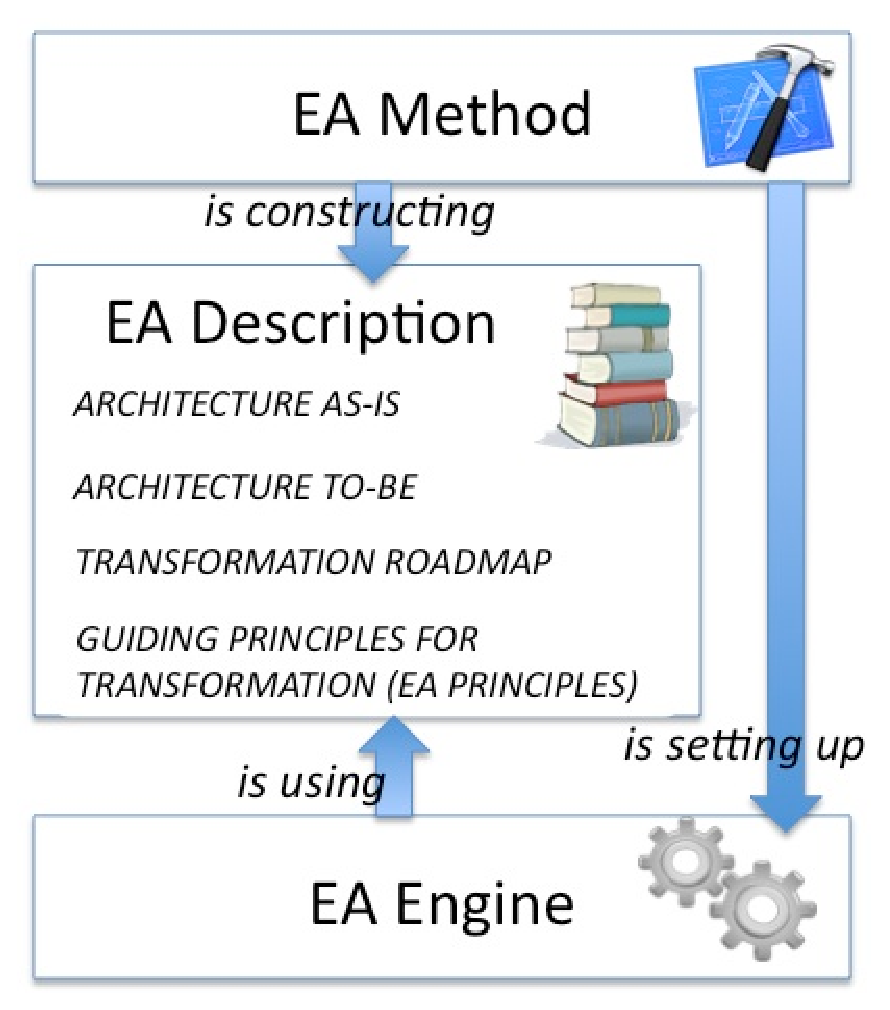
\includegraphics[scale=0.5]{EA}
\caption{Enterprise Architecture}
\label{fig:EA_general}
\end{figure}

%Enterprises are not alone in their trend towards decentralization; this trend also exists elsewhere. For example, peer-to-peer architectures -- where peers communication directly to each other, without the need for a central server -- are becoming increasingly popular.  These architectures now exist in many different areas, such as file sharing~\cite{bittorrent}, content distribution~\cite{blizzard}, revision control~\cite{progit}, as a digital currency~\cite{bitcoin2008}, for the funding of creative projects~\cite{kickstarter}, for moderation~\cite{reddit, slashdot}, and for content creation~\cite{wikipedia}. As a result, this thesis will look to take principles from peer-to-peer architectures and apply them to EA for increasing their support of decentralization. 




    \section{Problem}
    \label{sec:problem}    
    The problem of business-IT alignment is a relevant problem for all types of organizations, regardless of whether they have a centralized or decentralized structure. Solving it allows all components of an enterprise to operate together in a collaborative manner for the purpose of maximizing overall benefit to the enterprise. Enterprise Architecture frameworks outline a formal way in which to solve this problem. This thesis argues, however, that modern EA frameworks are primarily supportive of centralized organizations, and as such, have some shortcomings when applied in decentralized organizations. As modern organizations are becoming increasingly more decentralized, this suitability of modern EA frameworks for decentralization is becoming increasingly relevant. Consequently, this thesis addresses the problem of creating a suitable EA for decentralized organizations.

An important part of this thesis project is to analyze the suitability of existing EA frameworks for decentralization. Therefore, the problem will be fully explicated--including a precise definition, problem motivation, and root cause analysis--in the results chapter, Section \ref{sec:problem}.

    
    \section{Goals and Purpose}
    \label{sec:resq}
    The purpose of this thesis project is to contribute to the field of EA by improving it's support for decentralization. This is supported by two primary goals: The first goal is to demonstrate specific aspects of existing EA frameworks that are supportive and not supportive of decentralized organizations. The second goal is to contribute towards an EA framework supporting decentralization by design an artifact that overcomes a subset of the identified shortcomings.
        
    \section{Research Questions}
    \label{sec:resq}
    In order to adequately solve the problem presented in section~\ref{sec:problem}, this thesis will answer two research questions. The first question will address the problem of whether or not current Enterprise Architecture methods and frameworks are suitable for use in decentralized environments. The second question addresses the problem of creating an EA framework that is suitable for decentralized environments. Answering these two research questions will enable this thesis to make a contribution the field of EA by providing a basis for how EA can be extended to an area (i.e. decentralized organizations) where, currently, it is not typically applied. 

The two research questions for this thesis are:

\begin{enumerate}
\item What aspects of existing EA frameworks are supportive of decentralized organizations? What aspects are not supportive?
\label{req:1}
\item What are the principals of an EA framework that is supportive of decentralized organizations?
\label{req:2}
\end{enumerate}


    
    \section{Limitations}
    \label{sec:resq}
    Due to time constraints, this thesis project is not able to address the entirety of the problem identified. Instead, only a subset of identified issues with EA will be addressed. This is specific in Section \ref{sec:design}.
    
    \section{Chapter Layout}
    \label{sec:resq}
    This paper is structured as follows:
\begin{description}
  \item[Chapter 2 - Extended Background] An extended background on decentralization in organizations and on three modern EA frameworks is presented here. Additionally, the related subjects of Enterprise Integration and Enterprise modeling are covered as related works. 
  \item[Chapter 3 - Method] This chapter contains: a justification for following design science; the chosen research methods and strategies along with reasons for these choices and a discussion of alternatives; how these methods and strategies are actually applied for this research; and lastly ethical considerations are covered. 
  \item[Chapter 4 - Results] This chapter contains: an explication of the problem with how the EA frameworks of TOGAF, Zachman, and FEA support decentralization; an explication of the problem with the case organization's support for EA; an outline of the solution artifact, which takes the form of guidelines (part of Johannesson and Perjon's method artifact type~\cite[Ch. 2.4]{johannessonPerjons2012}), and its accompanying requirements; the design of the artifact, which was performed with the aid of knowledge on peer-to-peer architectures; a demonstration of the artifact based on a case study; and an argumentative evaluation of the artifact through it's demonstration.
  \item[Chapter 5 - Conclusions \& Discussions] This chapter describes the primary conclusions drawn from the results, a discussion of the validity of the results, a discussion of ethical and societal consequences, and recommendations for future works. 
\end{description}
    
    % Part 2, Scientific Base
    
    \chapter{Extended Background}
    \label{chap:extendedBackgrounf}
    
    \section{Enterprise Architecture}
    \label{sec:ea}
    
According to Sessions~\cite{sessions2007}, the field of Enterprise Architecture (EA) emerged in order to combat two increasingly prevalent problems facing enterprises: system complexity and business-IT alignment. As enterprises rely more and more on information systems of increasing complexity, these problems become even more important. The field of EA views the solution to these problems to be one of concurrent design. It is not enough simply try and fit IT to the business; business and IT aspects should be designed concurrently. 

While there is no singular agreed-upon definition for EA, different definitions\cite{jungle2004,GartnerInc,ross2006,pearlson2009,lankhorst2009,sessions2007,togaf9.1} do have much in common. EA is a discipline that takes a holistic approach to transforming high-level business vision and goals into the integration of an enterprise's organizational structure, business processes, and information systems. This transformation involves identifying and implementing the necessary change for this to occur. In order to view different EA frameworks from a common perspective, this thesis will break them down into three separate components that contribute to this transformation: the EA method, the EA description, and the EA engine (Figure \ref{fig:EA_general}). 

The Method aims to lay the groundwork for the EA project. Typically, this involves setting up teams, ownership, responsibilities and gaining commitment. Also it defines the overall process of collecting, validating and approving the EA artifacts  (e.g. descriptions As-Is, To-Be, gap analysis,  principles) that will form the second component - The EA description.  The Engine involves setting up a support structure for ensuring the ongoing adoption of the to-be EA description. This can involve gaining commitment fr  om stakeholders, setting up some compliance checking procedures, and deciding upon a prioritization of tasks to be completed. The remainder of this section will look at three different EA frameworks from the perspective of of these three phases: The Open Group Architecture Framework (TOGAF), the Zachman Framework, and the Federal Enterprise Architecture (FEA). These three frameworks were chosen as they are all well-known and accepted in the field of EA: In~\cite{sessions2007}, for example, Sessions estimates that TOGAF, Zachman Framework, and FEA (along with The Gartner Methodology) are used by 90 percent of the field.

\subsection{TOGAF}
The Open Group Architecture Framework, more commonly know as TOGAF, is a freely available EA framework created by The Open Group\footnote{~\url{www.opengroup.org}}, a consortium of IT organizations. TOGAF is comprised of a number of different aspects, mainly: the Architecture Development Method (ADM), ``a method for developing and managing the lifecycle of an enterprise architecture''~\cite[Ch. 5.1]{togaf9.1}; the Architecture Content Framework, a companion to the ADM which describes the content of the products of the ADM; the Architecture Landscape and Enterprise Continuum, which provide a means to organize the produced architectures; a set of reference models; and the Architecture Capability Framework, a set of ``reference materials'' for successfully operating an ``architecture function'' within an enterprise~\cite[Ch. 45]{togaf9.1}. 

%[SOMETHING ABOUT FLEXIBILITY AND ITERATION]
%
%3 levels of iteration:
%- multiple ADMs to create different architectures
%- within ADM
%- change
%
%ADM, Continuum,  \cite{lankhorst2009}

% this thesis argues that TOGAF is primarily supportive of centralized orgs -> contribution is to identify a way to adapt it to decentralized

\subsubsection{EA Method}
The TOGAF ADM falls under our EA Method component of EA. The TOGAF ADM is made up of a preliminary phase, six core phases (labeled A-H), and a requirements management component. 

\begin{figure}
\includegraphics[scale=0.7]{ADM}
\caption[TOGAF: ADM basic structure]{TOGAF: ADM basic structure \cite[Sec. 5.2.2]{togaf9.1}}
\label{fig:ADM}
\end{figure}

In TOGAF, the preliminary phase lays the groundwork for the rest of the EA process. Some important aspects are to set up a governance structure and EA team for the EA process and to establish a repository for storing all architectural information~\cite[Ch. 6]{togaf9.1}.

Phase A of the TOGAF Process, the architectural vision phase, is aimed at setting a clear vision for the enterprises future architecture. This involves creating the initial as-is architecture as well as setting clear, management approved goals and requirements, and transforming them into a high-level vision of the enterprises to-be architecture~\cite[Ch. 7]{togaf9.1}.

At this point, TOGAF suggests that the outputs of the preliminary phase and phase A be organized into a ``Statement of Architecture Work''. This document is to be approved by project sponsors~\cite[Sec. 7.4.11]{togaf9.1} and can be used to form the basis of a contract between the architecture provider and the client~\cite[Sec. 36.2.20]{togaf9.1}.

The next three phases, B-D are concerned with creating the as-is and to-be business architecture, information systems architecture, and the technology architecture~\cite[Ch.8-12]{togaf9.1}. TOGAF suggests two different approaches to creating the architectures: baseline first or target first~\cite[Ch. 19.4]{togaf9.1}. Baseline-first involves analyzing the as-is architecture for areas where improvements can be made. Target-first aims at creating a detailed target architecture and then mapping it back to the as-is architecture in order figure out what needs to change. The main aspects of these phases are to develop the as-is and to-be architectures, analyze the gap between them, and create an initial road-map of the steps needed to cross the gap.

Phase E and F, Opportunities and Solutions and Migration Planning, are concerned with organizing the work to be done into projects, and then creating a schedule for executing the projects~\cite[Ch. 13-14]{togaf9.1}.

Phase G is concerned with the implementation and setting up a framework for its governance and its compliance to the target architecture~\cite[Ch. 15]{togaf9.1}.

%mention H is part of engine?

\subsubsection{EA Description}
TOGAF views architecture from the perspective of four different architecture domains~\cite{sessions2007}: business, application, data, and technical. Business architecture is concerned with processes and functions used to meet business goals, application architecture is concerned with the design of specific applications and their interactions, data architecture is concerned with managing enterprise data, and the technical architecture is concerned with the infrastructure (hardware and software) used to support the applications. The architectures in these four domains are created through the ADM phases B (Business Architecture Phase), C (Information Systems Architectures Phase) and D (Technology Architecture).

\paragraph*{Architecture Landscape}
The various architectural artifacts in TOGAF are organized across an Architectural Landscape~\cite[Ch. 20]{togaf9.1} of three dimensions: breadth, level, and time. Breadth refers to the area of subject matter for an architecture. Levels refer to the level of detail of an architecture. TOGAF specifies three levels of detail: strategic, for overall direction setting at the executive level; segment, for architectures at the level of a program or portfolio; and capability, for architectures concerned with how the architecture process is itself enabled and governed. The time dimension of the landscape keeps the state of architectures as they evolve over time. Additionally, the Architecture Landscape can be partitioned into independent partitions for supporting different organizational units~\cite[Ch. 40]{togaf9.1}. 

%Breadth: The breadth (subject matter) area is generally the primar y organizing character istic for descr ibing an Architecture Landscape. Architectures are functionally decomposed into a hierarchy of specific subject areas or segments.

%Capability Architecture provides an organizing framework for change activity and the development of effective architecture roadmaps realizing capability increments.

\paragraph*{Enterprise Continuum}
At each level of the Architecture Landscape, architectures are further organized through the Enterprise Continuum which provides a way to organize the architectures from generic to organization-specific~\cite[Ch. 39]{togaf9.1}. The most generic are called Foundation Architectures~\cite[Ch. 39.4.1]{togaf9.1}, which are applicable to all enterprises. A core aspect of a Foundation Architecture is to provide a high-level taxonomy which can provide a basis for the more specific architectures~\cite[Ch. 43]{togaf9.1}. 

The second set of architectures in the continuum are called the Common Systems Architectures~\cite[Ch. 39.4.1]{togaf9.1}. These architectures are specific to a generic problem domain (e.g. security management), and are thus applicable to a wide range (but not all) of enterprises.

The third set of architectures in the continuum are called Industry Architectures. These architectures are applicable to a specific problem within a specific industry. They are thus useful to many members of that industry, but not necessarily outside of it. The most specific level in the continuum are Organization-Specific  architectures. As the name implies, they are relevant only to a specific enterprise. These outline the architectural solution for a particular enterprise and provide "a means to communicate and manage business operations across all four architectural domains"~\cite[Ch. 39.4.1]{togaf9.1}.

\paragraph*{Reference Models}
TOGAF includes two reference models. The Technical Reference Model (TRM) is a Foundation Architecture which describes a number ``of generic services and functions that provides a foundation on which more specific architectures and architectural components can be built'' ~\cite[Sec. 43.1.1]{togaf9.1}. The second provided reference model, the Integrated Information Infrastructure Reference Model (III-RM), is a subset of the TRM and is classified as a Common System Architecture on the Enterprise Continuum~\cite[Ch. 44]{togaf9.1}. The III-RM is a reference model for enabling information integration across an enterprise. 

%The content of TOGAF architecture artifacts is defined in the Content Framework... [Still don't really understand this part] [maybe content is actually determined through reference models which are placed on the continuum?]

% architecture partitioning
% architecture capability

\paragraph*{Architecture Content Framework}
The Architecture Content Framework (ACF) describes the outputs of the architecture efforts from the TOGAF's method, the ADM. The content of the outputs is described by the Content Metamodel~\cite[Ch. 34]{togaf9.1}, which is summarized in Figure~\ref{fig:togaf_content}. The outputs can are seen from three different viewpoints~\cite[Ch. 4]{Bente2012} described by the content framework: deliverables, artifacts, and building blocks~\cite[Ch. 33]{togaf9.1}. A \textit{deliverable} is an output that is specified in the architecture contract, and is therefore subject to formal review and sign-off. A deliverable is composed of one or more \textit{artifacts} which describe some aspect of the architecture. Artifacts, in turn, describe \textit{building blocks}, which represent either: a) a specific functionality of the enterprise, or b) an actual component which implements a specified functionality.

\begin{figure}
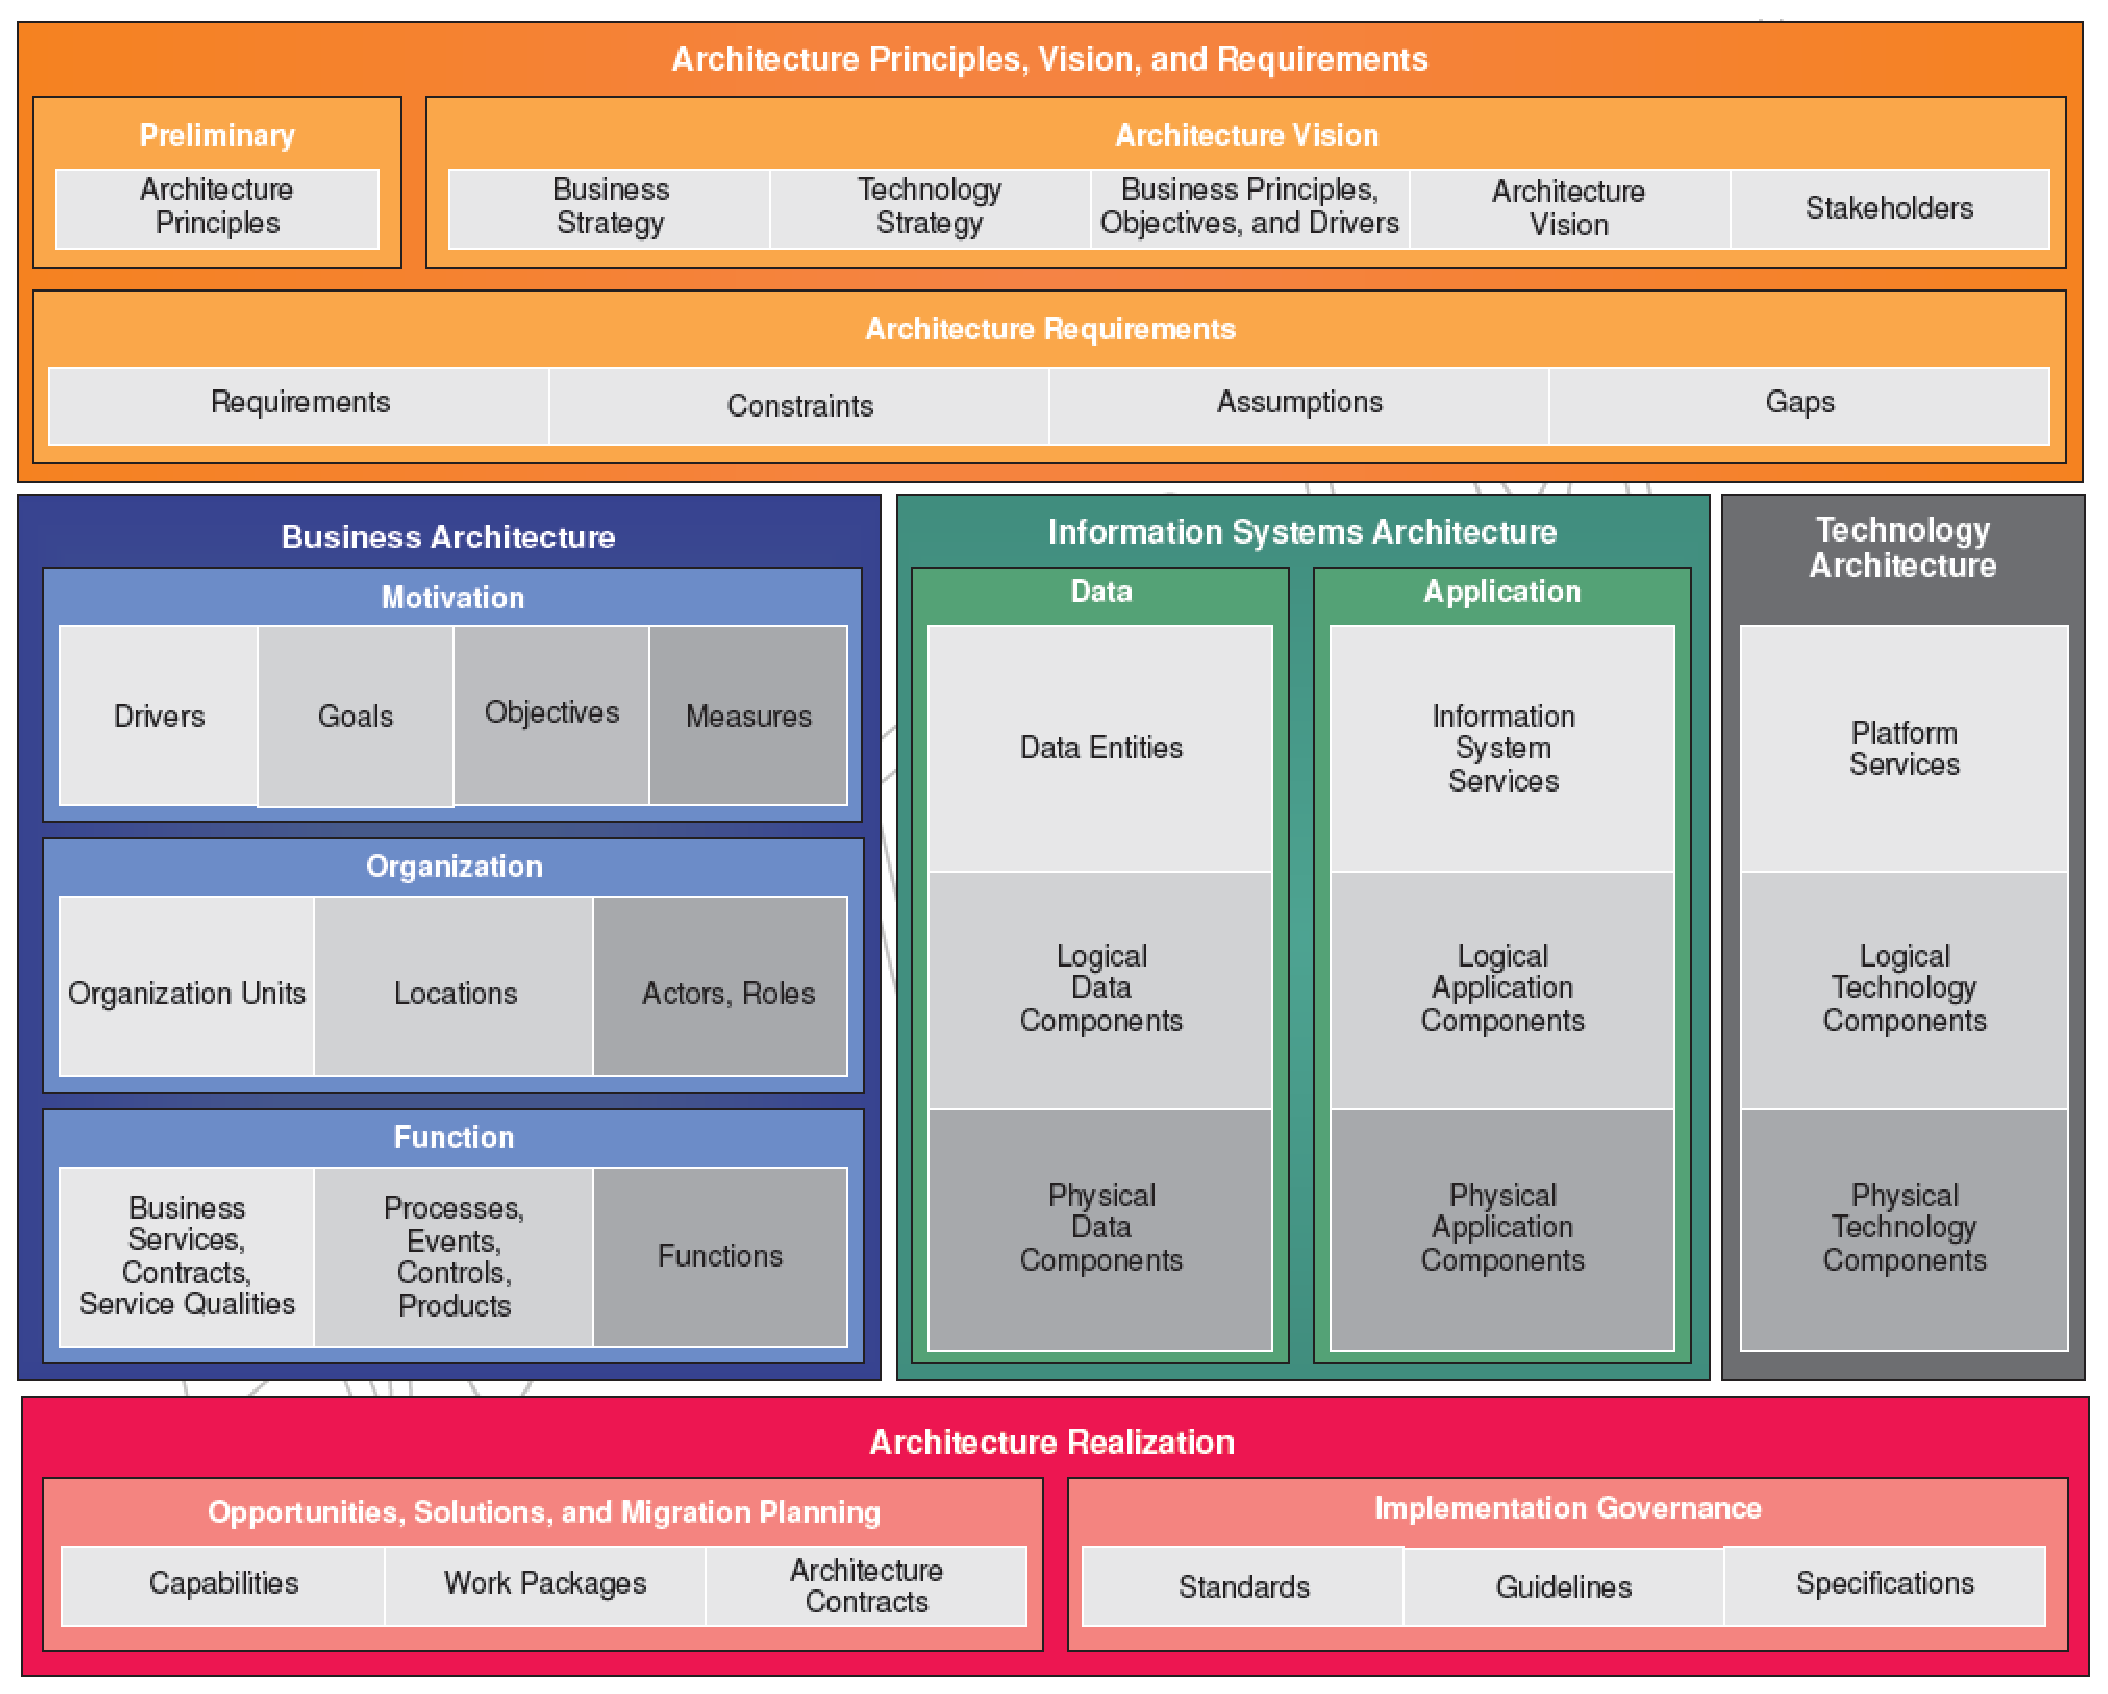
\includegraphics[scale=0.3]{togaf_content}
\caption[TOGAF: Content Metamodel]{TOGAF: Content Metamodel~\cite[Sec. 34.2]{togaf9.1}}
\label{fig:togaf_content}
\end{figure}

\subsubsection{EA Engine}

The engine component TOGAF is composed of an on-going change management process and a framework for managing architecture capability in an enterprise.

\paragraph*{Architecture Change Management}

The final ADM phase, phase H, outlines an ongoing change management process for the architecture of an enterprise.  It is concerned with managing changes to the architecture throughout its lifecycle~\cite[Ch. 16]{togaf9.1}. In this phase, a governance body sets criteria for determining if a change requires an architecture update if a new cycle of the ADM needs to be started. An important aspect of this process is to deploy tools for monitoring for business and technological changes and measuring performance indicators. 

\paragraph*{Architecture Capability Framework}

TOGAF describes its Architecture Capability Framework as providing a set of reference materials for creating appropriate ``organization structures, processes, roles, responsibilities, and skills'' in order to ``successfully operate an architecture function''~\cite[Sec. 45.1]{togaf9.1}. Key components of this framework are the creating of an Architecture Board, a formal architecture compliance process, the use of architecture contracts, and guidelines for architecture governance. 

The Architecture Board is responsible for overseeing architecture governance activities. Specific responsibilities include ``[p]roviding the basis for all decision-making with regard to the architectures'', ensuring the various partitioned architectures are consistent, and enforcing compliance~\cite[Ch. 47]{togaf9.1}. 

TOGAF describes a formal review process for determining compliance. The main goal of this process is to ``[f]irst and foremost, catch errors in the project architecture early, and thereby reduce the cost and risk of changes required later in the lifecycle''~\cite[Ch. 48.3.1]{togaf9.1}. This process is outlined in Figure~\ref{fig:togaf_compliance}.

\begin{figure}
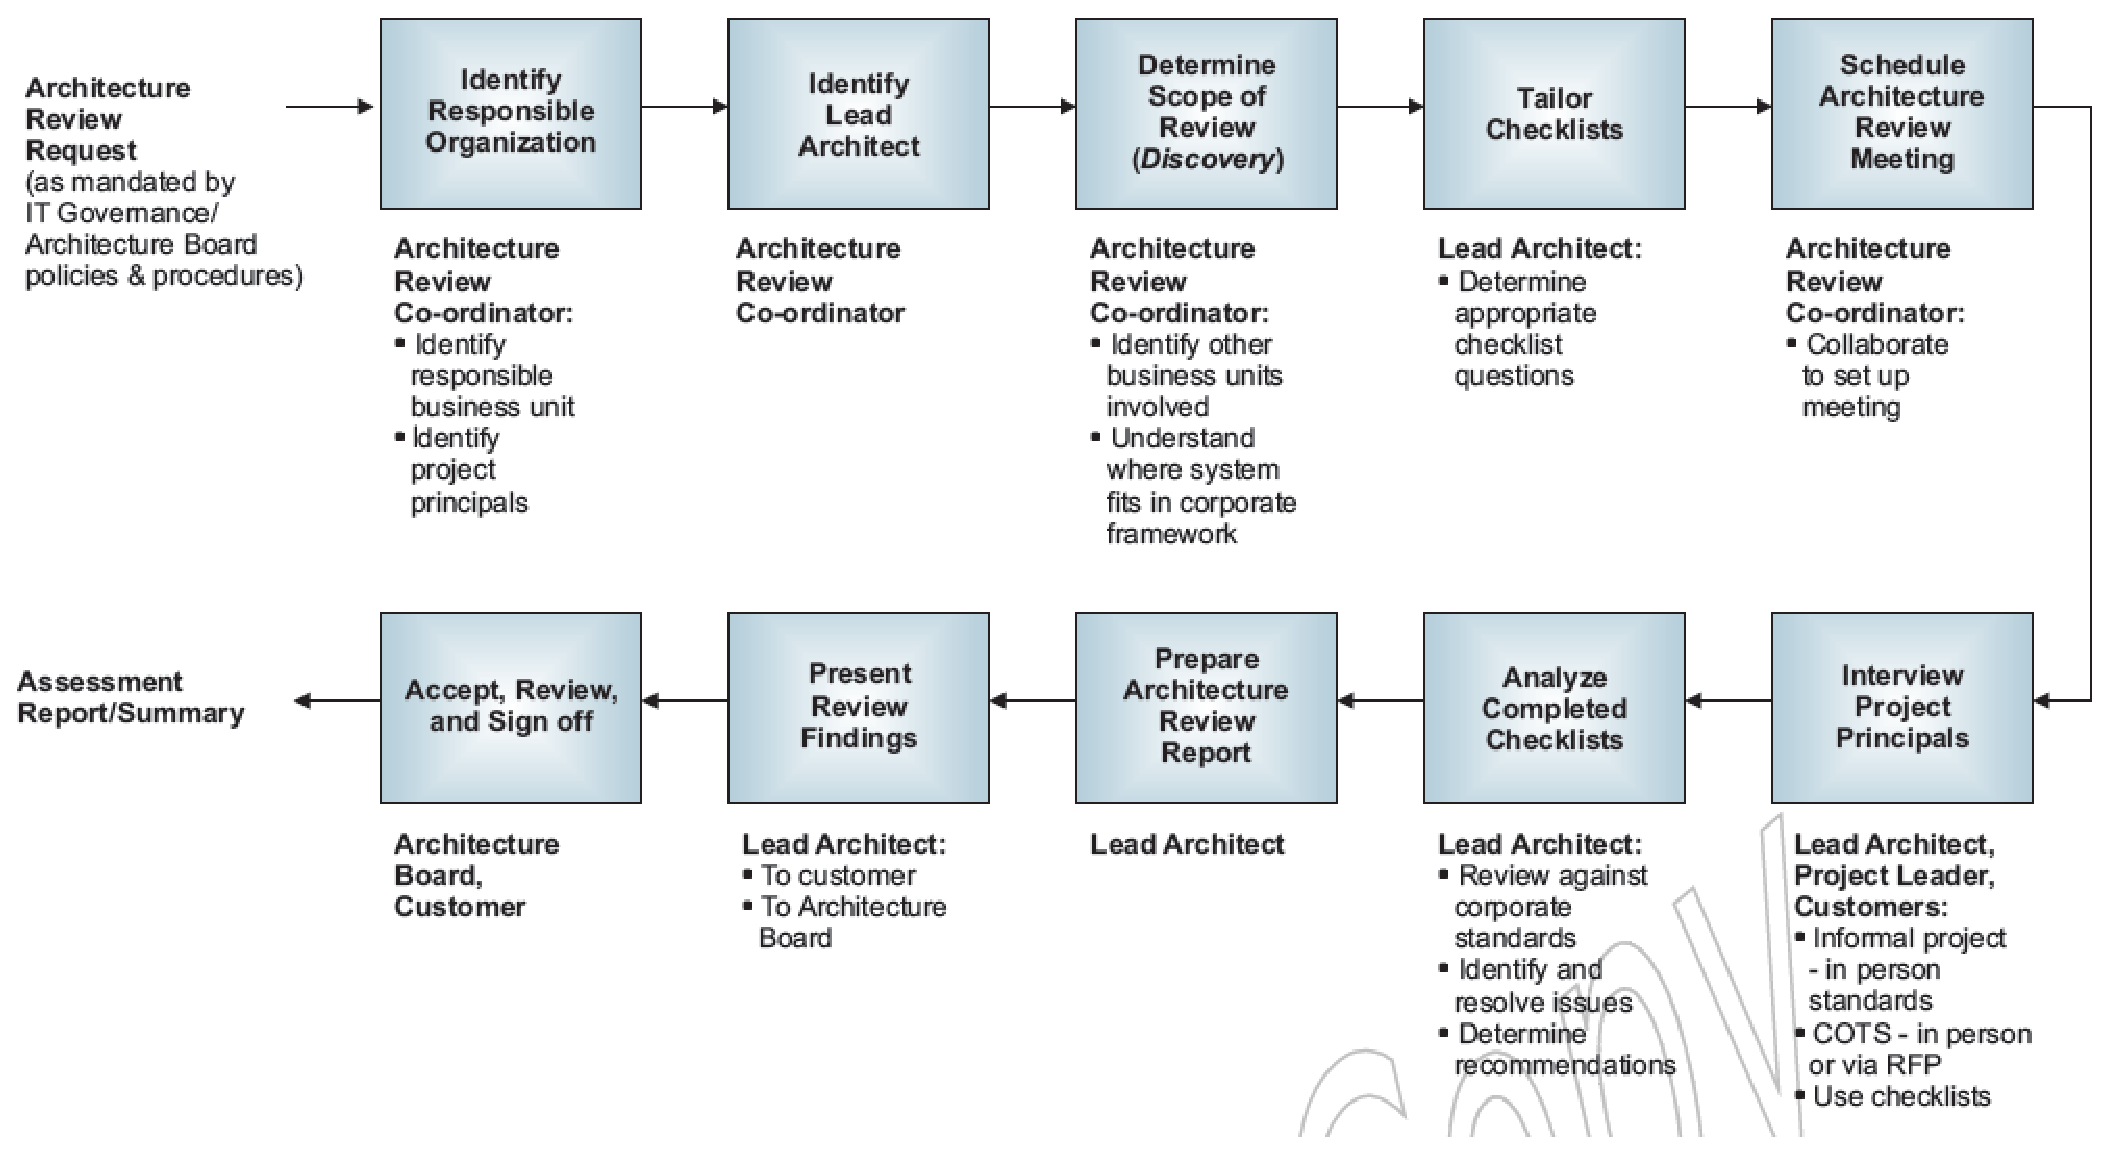
\includegraphics[scale=0.3]{togaf_compliance}
\caption[TOGAF: Architecture Compliance Review Process]{TOGAF: Architecture Compliance Review Process~\cite[Sec. 48.4.1]{togaf9.1}}
\label{fig:togaf_compliance}
\end{figure}

% this diagram has strict roles

%Some other goals of this process are to "Ensure the application of best practices to architecture work" "Provide an overview of the compliance of an architecture to mandated enterpr ise standards." "Identify where the standards themselves may require modification." "Communicate to management the status of technical readiness of the project." "Identify and communicate significant architectural gaps to product and service providers"

TOGAF suggests the use of contracts between architecture developers and sponsors (i.e. the party who wants the architecture) in order to have a formal agreement on the ``deliverables, quality, and fitness-for-purpose''~\cite[Ch. 49]{togaf9.1}. The goal of having contracts is to guarantee: continuous monitoring of architecture decisions, changes, and integrity; adherence to architecture ``principles, standards and requirements''; that all risks are identified;  the existence of processes to ensure ``ensure accountability, responsibility, and discipline''; and a formal definition of governance and decision making authority. Adherence to the contracts is guaranteed by architecture governance.

In TOGAF, ``architecture governance is an approach, a series of processes, a cultural orientation, and set of owned responsibilities that ensure the integrity and effectiveness of the organization's architectures''~\cite[Ch. 50]{togaf9.1}.The suggested organizational structure for governance involves three separate phases--Develop, Implement, and Deploy--supported by the Enterprise Continuum, and overseen by a CIO/CTO. In order for the architectural effort to be successful, the architecture governance strategy needs to specify an Architecture Board, a set of architecture principles, and ensure compliance.  %This is visualized in Figure~\cite{togaf_govStructure}.
%
%\begin{figure}
%\centering
%\includegraphics[scale=0.2]{togaf_govStructure}
%\caption{TOGAF: Architecture Governance Framework -- Organizational Structure from \cite[Sec. 50.2.2.1]{togaf9.1}}
%\label{fig:togaf_govStructure}
%\end{figure}

\subsection{The Zachman Framework}

The Zachman Framework was the first EA, first introduced by John Zachman in 1987~\cite{sessions2007,zachman}. It consists only of a taxonomy, and as such only fits into the EA Description aspect of EA. 

\subsubsection{EA Method and Engine}

Despite not specifying an engine or method for use with ZF, these components are still necessary for a successful EA effort. ZF can be used however an organization wishes, though some formal guidelines do exist for its use. One option is to fit ZF into another EA framework, replacing that framework's EA description with ZF. TOGAF, for example, states that it is possible to replace the TOGAF content framework with ZF~\cite[Ch. 33]{togaf9.1}. A second option is pay for formal training from Zachman International~\cite{zachmanInc}, where it is possible to get certified in the use of ZF. A third option is through hiring a consultant who is already familiar with ZF. Zachman International, for example, offers consulting services.

\subsubsection{EA Description}

The Zachman Framework (ZF) breaks down EA into a grid of perspectives. Each perspective is characterized by two things; its target audience and the issue is aimed at. ZF covers six issues: What (data and entities), How (functional), Where (locations and interconnections/networks), Who (people relationships), When (events and performance criteria), Why (motivations and goals)~\cite{jungle2004}. For each issue, it views it from six different perspectives: executive, business management, architect, engineer, technician, and enterprise users. 

The executive perspective is meant for executives or planners and needs to provide an estimate of a system's functionality and cost~\cite{jungle2004}. The business management perspective is a business view of how an owner thinks the business operates~\cite{Zachman2000}. The architect perspective takes a systems viewpoint and describes the operations and interactions of the variety of systems in an enterprise. The engineer perspective views describes the physical technology and design of the individual systems. The technician perspective takes the perspective of a "sub-contractor" who is implementing a specific system and the high, out-of-context level of detail associated with that. The enterprise users perspective describes the perspective of the people who actually use the system. 
 
%[XXXX Zachman Diagram XXXX]

\subsection{Federal Enterprise Architecture}
The Federal Enterprise Architecture (FEA) is an effort by the federal government of the United States to create an EA for the entire government. The FEA is a complete EA framework, covering all three components of EA. The Federal Enterprise Architecture Program Management Office describes FEA as ``...a common language and framework to describe and analyze IT investments, enhance collaboration and ultimately transform the Federal government into a citizen-centered, results-oriented, and market-based organization as set forth in the President's Management Agenda.''~\cite{FEA_PMO2007} FEA takes takes an approach where individual organizational units develop their own architectures that fit into an overall framework of common standards and interoperability.

FEA is composed of six core elements~\cite{sessions2007}:
\begin{itemize}
    \item The organization is broken-down into different segments of varying scopes, and architecture is developed for each segment
    \item A set of five reference models which are used as a basis to describe the important elements of the FEA in a consistent manner
    \item A process for creating each segment EA
    \item A transitional process for moving from the current state of the enterprise to the visioned state
    \item A taxonomy for organizing the various assets of the FEA
    \item Guidelines for measuring the degree of success of the FEA
\end{itemize}
Compared to TOGAF and Zachman Framework, FEA defines both the taxonomy for EA artifacts (EA description in Fig. \ref{fig:EA_general} ) and the EA process for creating these artifacts and using them by organization (EA method and EA engine in Fig.\ref{fig:EA_general} ). 

\subsubsection{EA Description}
% ~\cite{sessions2007}
FEA develops architecture for segments and enterprise services. A segment is a ``major line-of-business functionality''~\cite{sessions2007} for an individual organizational unit (such as an agency or department). Two types of segments exist: core mission-area segments and business service segments~\cite{FEA_PMO2007}. Core mission-area segments are at the scope of a single organizational unit (though they may be shared by different units) and are essential to its purpose~\cite{sessions2007,FEA_PMO2007}. Business service segments are also at the scope of an individual organizational unit, however these segments exist in all organizational units and are defined for the entire enterprise. Like business service segments, enterprise services are defined organization-wide. However, they are different in that they also function at the enterprise level, e.g. a single security management service that is shared by the entire enterprise. 

The EA artifacts defined by FEA include  baseline segment architectures, target segment architectures and transition strategy. The EA transition strategy describes the overall plan and schedule to achieve the target (``to-be'') architecture.

%Segment identification is a continuous, iterative process. Enterprise assets including systems and IT investments are mapped to the agency-level reference models to create a segment-oriented view of the enterprise (see Figure 2-2). 
%
%"The FEA consists of a set of interrelated "reference models" designed to facilitate cross-agency analysis and the identification of duplicative investments, gaps, and opportunities for collaboration within and across agencies. Collectively, the reference models [compose] a framework for describing important elements of the FEA in a common and consistent way."~\cite{FederalEnterpriseArchitectureProgramManagementOffice}
%
%"This, in a nutshell, is the goal of the five FEA reference models: to give standard terms and definitions for the domains of enterprise architecture and, thereby, facilitate collaboration and sharing across the federal government."

In order to have a common language for describing the enterprises assets, FEA describes five reference models for mapping assets to segments and enterprise services~\cite{FEA_PMO2007}. The five reference models are the performance reference model, the business reference model, the service component reference model, the technical reference model, and the data reference model. 
%\begin{figure}
%\centering
%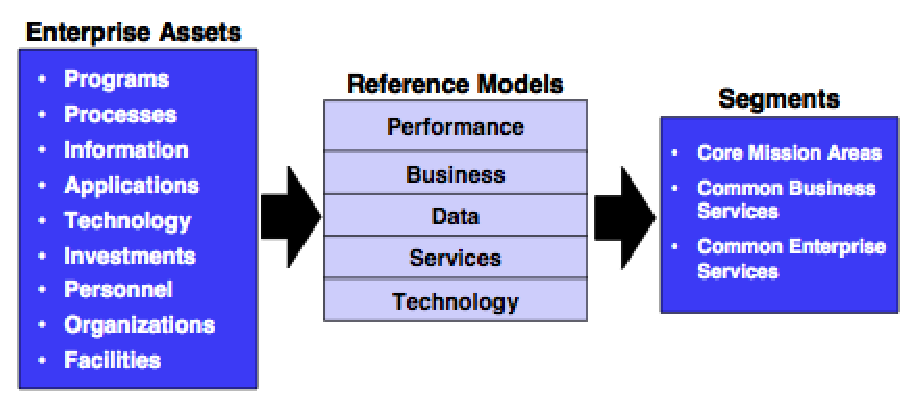
\includegraphics[scale=0.6]{FEAsegm}
%\caption{FEA: Segment Identification from ~\cite{FEA_PMO2007}}
%\label{fig:FEA_segmentID}
%\end{figure}
%[Insert Segment Identification Figure (2.2 on page 20 of ~\cite{FederalEnterpriseArchitectureProgramManagementOffice} )]

The performance reference model provides a framework for developing consistent measurement. The business reference model provides a framework for developing a functional view of the enterprises line of business. The service component reference model provides a framework for describing how the services offered by IT systems support business functionality.  The data reference model provides a framework for describing data in a consistent way that enables enterprise-wide sharing. 

\subsubsection{EA Method}

% Performance Improvement Lifecyle seems to be the overall FEA process

%"single agency contains both core mission area segments and business service segments. Enterprise services are those cross-cutting services spanning multiple segments."\cite{FederalEnterpriseArchitectureProgramManagementOffice2007}
%"By contrast, segment architecture defines a simple roadmap for a core mission area, business service or enterprise service"~\cite{FederalEnterpriseArchitectureProgramManagementOffice2007}
%
% ~\cite{sessions2007}
%
%Segments 
% - segment is a major line-of-business functionality, e.g. HR
%     - core mission-area segments, central to mission/purpose of organization
%     - business-services segment, foundational to all organizations
% - function at agency level, defined at enterprise level

% Just as enterprises are themselves hierarchically organized, so are the different views provided by each type of architecture.
 
FEA defines a four step iterative process for creating architectures for each segment and service~\cite{FEA_PMO2007}:
\begin{enumerate}
    \item Architectural analysis
    \item Architectural definition
    \item Investment and funding strategy
    \item Program management plan and execute projects
\end{enumerate}

%New and revised business and information requirements are continuously identified as the segment moves though each lifecycle phase, and as business and information management solutions are funded and developed to meet stakeholder requirements. Consequently, segment architecture work products must be maintained to reflect these inputs.

The first step, architectural analysis, is concerned with defining the scope of the segment, its baseline architecture, current problems in the segment, and a high-level vision of the desired final state for the segment~\cite{FEA_PMO2007}.

The second step, architectural definition, is concerned with defining the detailed target architecture of the segment~\cite{FEA_PMO2007}. Aside for the architecture itself, it is also necessary to define a roadmap of projects to get there, the segment transition strategy, and the performance goals of the architecture. 
  
The third step, the investment and funding strategy, is concerned with specifying how the projects identified in the segment transition strategy are to be funded~\cite{FEA_PMO2007}. 

The fourth step, program management plan and execute strategies, is concerned with making detailed plans for the individual projects, executing the plans, and defining performance measurements for the initiative~\cite{FEA_PMO2007}.
%\begin{figure}
%\centering
%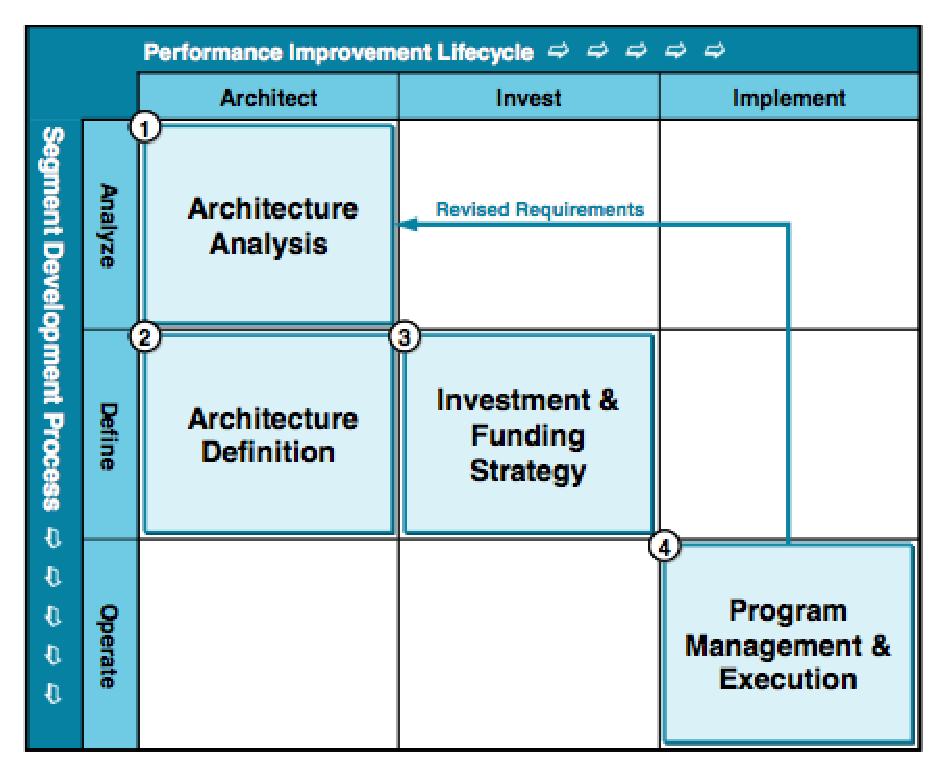
\includegraphics[scale=0.4]{FEA}
%\caption{FEA: Segment Architecture Development and Maintenance from ~\cite{FEA_PMO2007}}
%\label{fig:FEA_segmentDev}
%\end{figure}
%[Insert Figure 3-2: Segment Architecture Development and Maintenance from ~\cite{FEA_PMO2007}]

% is there an EA agency???
    
\subsubsection{EA Engine}
%~\cite{sessions2007}

FEA describes an activity to maintain the architecture in order ensure that it stays relevant over time. FEA calls this activity ``segment architecture maintenance''~\cite{FEA_PMO2007}. In this activity, it is important to monitor for, list and prioritize new architectural change drivers as they appear. The impact of these drivers needs to be defined. 

% term is "architectural change drivers.", maybe define

% Performance Improvement Lifecycle
FEA  defines  an EA value measurement process: ``a continuous, customer- focused process relying on feedback from EA stakeholders and other value measures to increase the quality and effectiveness of EA products and services to support business decisions''~\cite[Sec. 5]{FEA_PMO2007}.

FEA describes ``EA governance and management processes''~\cite[Sec. 2]{FEA_PMO2007} to control architecture development. These process are implemented to manage standards, enforce compliance, manage collaboration between agencies, approve architectures for implementation, and  manage business and IS requirements for managing EA change.

%Segment architecture development is controlled by EA governance and management
%processes across each phase of the Performance Improvement Lifecycle. Governance
%and management processes are implemented to:
%• Review segment architecture work product content and format standards to
%promote reconciliation with the agency EA and relevant cross-agency initiatives;
%• Validate opportunities for agency-level and cross-agency collaboration and reuse
%including the implementation of relevant cross-agency initiatives;
%• Review and approve segment architecture in advance of IT investment and
%project execution;
%• Capture segment-level business and information management requirements to
%update and maintain the agency EA; and
%• Capture lessons learned to improve the segment architecture process and
%standard work products.
%
%
%In addition to the segment architecture maintenance activity, the Office of Management and Budget (OMB) describes an "Enterprise Architecture Assessment Framework" for the continuous assessment of each agencies performance in their EA practice~\cite{OfficeofManagementandBudget}. This framework assesses the maturity of the enterprises adoption of EA in three dimensions of KPIs: completion, use, and results. The "completion" dimension aims to measure the completeness of an agencies target EA and transition plan, i.e. how well it is "positioned to serve  as the agency's blueprint that describes its future state from a performance, business, service, data, and technology standpoint"~\cite{OfficeofManagementandBudget}. The "use" dimension measures how well the architecture is used to "drive decision making"~\cite{sessions2007}. The results dimension measures the direct benefits of using the architecture~\cite{sessions2007}, such as measurable improvements in the performance of programs or the direct benefits to decision makers~\cite{OfficeofManagementandBudget}. 



%[Insert Figure 2-1: Information and IT-Enabled Performance Improvement Lifecycle from~\cite{OfficeofManagementandBudget}]

% \subsection{A Reference Architecture for Collaborative Networks (ARCON)}

% Move to a related work








    
    \section{Decentralization in Organizations}
    \label{sec:organizations}
    This section will first discuss the forms of organizational structure defined in the literature. Second, the (de)centralization of current organization and, as a consequence, their styles of IT governance will be explored. We conclude this section by underpinning the challenges organizations have to face due to their progressive decentralization.

\subsection{What is a Decentralized Organization?} 
 
An organization can be structured in many different ways. Sachdeva \cite{sachdeva1990} defines organizational structure as "... institutional arrangements and mechanisms for mobilizing human, physical, financial and information resources at all levels of the system..." According to Jacobides \cite{jacobides2007}, "Organizational structure provides the frames through which individuals see their world. Thus, the way each organization is structured shapes an ecology of different, distinct frames that exist at the level of the organizational subunit." 
%Nystrom and Starbuck \cite{nystrom1981} define organisational structure as the arrangement and interrelationship of component parts and positions in an organization.

There has been a lot of research on specific forms of organizational structure. Taxonomies of organization forms are defined in  \cite{mckelvey1982}, \cite{rich1992}.   \textit{Classic} and \textit{modern} types of organizational structure are often recognized.  Classic types include simple centralized organizations ~\cite{Mintzberg1979}, bureaucratic organizations \cite{mintzberg1981}, divisional structure and functional structure. Modern  types include matrix structure, flat organizations, adhocracy. New forms of organizational structure emerged recently: collaborative networks, virtual organizations and coopetition.

According to Robbins \cite{robbins1997}, organizational structure has three components: complexity, formalization and centralization.  Complexity refers to the degree to which activities within the organization are differentiated; Formalization refers to the degree to which work is standardized; Centralization refers to the degree to which decision making is concentrated at one point in the organization. 

Following Luthens \cite{luthans2006}, centralization and decentralization can be also defined according to three factors: geographical or territorial concentration or dispersion of operations; functions;  extent of concentration or delegation of decision making powers. In \cite{pearlson2009},  the following characteristics of centralization are defined: the allocation of decision rights,  the structure of communication lines and  the choice of forms of coordination.

In a centralized organization, all decision making authority would reside with a single, top-level authority. In a completely decentralized enterprise all members would have equal decision making rights. Here, hierarchy manages the inter-dependencies between the different subunits of organization and often makes direct interactions and communications unnecessary \cite{thompson1967}.  Decentralized organizations instead have less formalized communication lines~\cite{pearlson2009, ahuja1998network}, and more fluid, project oriented teams.~\cite{applegate1988}

Centralized organizations lean towards primarily vertical style of coordination~\cite{Bolman2008}, which is characterized by formal authority, standardization and rules in operations and in IT, and planning and control systems. Decentralized organizations lean towards lateral coordination characterized by meetings, task forces, coordinating roles, matrix structures, and networks~~\cite{Bolman2008}. 

Below, popular forms of organizations focusing on their degree of centralization will be considered. 

\subsection{Forms of Organizational Structure and Decentralization}

\subsubsection{Classic Organizational Structures}

Pearlson and Saunders offer a thorough description of a pure hierarchical organization structure~\cite{pearlson2009}: Except for the top level position, each position has one superior and zero or more subordinates. Decision rights and communication lines are strictly defined and work their way down from the top (i.e. the center). The scope of a position is specialized and strictly defined by your superior and one works in assigned teams. The primary benefit of a hierarchy is that the high levels of management have strict governance and control over the company. Hierarchical organization structures are suited for stable, certain environments. 

Hierarchical organizations can be subdivided into simple centralized and bureaucratic organizations:

In simple centralized organizations, both strategic planning and operational decision making authority belongs to one person at the top. This structure can be found in small and single-person-owned organizations with only two hierarchical levels. 

Bureaucratic organizations \cite{mintzberg1981} are characterized by multi-level hierarchical structure and use of standard methods and procedures for performing work. 

Hierarchical organizations generally divide their labor either in terms of function, a grouping of common activities, or in terms of division, a grouping based on output (product). Two organizational structures, divisional and functional, can be identified accordingly.

\subsubsection{Modern Organizational Structures}

Matrix structure is another popular style of organization structure~\cite{pearlson2009} that can be seen as a mixture of functional and divisional structures. In this form, individuals are assigned two or more supervisors covering different (usually product and functional) dimensions of the enterprise. Pearlson and Saunders state that matrix organization structures are suited for dynamic environments with lots of uncertainty, presumably because their authority structure allows them to cover multiple aspects when making decisions. However, like a hierarchical structure, a matrix structure is a rigid construct with strictly defined roles, communication lines and decision rights. Authority still comes from the top in a centralized manner, even though it becomes more distributed among matrix managers at the lower levels~\cite{pearlson2009}. 
%Consequently, matrix structures still may not be perfectly suited for uncertain, dynamic environments. 

%Applegate, Cash, and Mills~\cite{applegate1988} support this statement, as they describe hierarchical and matrix structures as rigidly structuring "communication, responsibility, and accountability to help reduce complexity and provide  stability". They furthermore state that both matrix and hierarchical structures have the effect of stifling creativity and preventing organizations from being able to adapt effectively to rapidly changing environments. 

Flat organization is a novel type of organizations where only one or maximum two hierarchical levels are defined (similarly to simple centralized organizations). For example, Valve Corporation, a software company in the video game industry released their handbook in 2012~\cite{valveHandbook}.  Unlike simple centralized organization described above, individual employees have complete freedom despite there being a president/founder at the top: Nobody reports to anyone, and everyone is free to work on whatever they want to. This is an example of high decentralization.

Adhocracy~\cite{applegate1988,pearlson2009}  aims to discard traditional hierarchies in favor of decentralized decision rights and flexible communication lines connecting the entire enterprise. Specifically, instead of hierarchies, an adhocracy has a rapidly changing set of project oriented groups that have decision making authority and other powers  \cite{robbins1997}. Mintzberg describes an adhocracy as "a loose, flexible, self-renewing organic form tied together mostly through lateral means"~\cite{Mintzberg1979}.  

\subsubsection{Post-Modern Organizational Structures}

New forms of organizational structure enabled uniquely by modern information and communication technologies  Internet emerged recently:  collaborative networks~\cite{Camarinha-Matos2005} and coopetitions~\cite{Bengtsson2000}.

%Network organizations are characterized by subcontracting  their business functions \cite{????};

Related to the idea of adhocracy, is the concept of collaborative networks (CN). Camarinha-Matos and Afsarmanesh define collaborative networks as being composed of ``a variety of entities (e.g., organizations and people) that are largely autonomous, geographically distributed, and heterogeneous in terms of their: operating environment, culture, social capital, and goals.''~\cite{Camarinha-Matos2005} Three common characteristics in various CNs are autonomy in the individual entities, a drive towards meeting common or complementing goals, and the use of an agreed-upon framework for collaboration. 

Under the umbrella of CNs, Camarinha-Matos and Afsarmanesh define virtual organizations, virtual communities, and virtual breeding environments~\cite{Camarinha-Matos2005}. Virtual organizations are a group of independent organizations working together to achieve some goal(s); virtual communities are communities of individuals that interact with each other through the use of computer network-based technologies; and virtual breeding environments are frameworks for interoperability set up by groups of organizations in order to enable the potential for forming a virtual organization.

%These entities collaborate through  computer networks in order to achieve common or complementary goals. The main driver behind CNs is that the goals the seek to achieve would be impossible or much more difficult to achieve without collaboration. %The composition of autonomous entities makes CNs a very relevant concept to decentralization. 

Another organizational form emerged recently is coopetition. Bengsston and Kock describe coopetition as a complex relationship between firms where they simultaneously compete and collaborate and benefit from both~\cite{Bengtsson2000}. Coopetition allows the participating organizations to take advantage of a heterogeneity of resources. Organizations may seek to create competitive advantage through a unique resource they own (e.g. skill). At the same time, it might be beneficial for them to cooperate with another organization that possesses a unique resource that is of value to them. 

Virtual organizations and coopetitions differ from the organizational structures defined above since they do not represent a single legal entity but a group of autonomous and independent entities with different (and possibly concurrent) strategic goals. These entities are engaged into collaboration in response to factors such as specific market situations, customer demand, etc.  The heterogeneous structure of such organizations remains invisible for a customer, while the service level agreements should be maintained at the same high level any other organization would maintain. Such organizational structures are grounded on a sustainable collaboration between partners without any centralized control.

%They explore the concept of coopetition in the context of competing firms that "produce and market the same product".~\cite{Bengtsson2000} In this context, they place an important limit on coopetition: their needs to be some kind of separation between the competing and cooperating aspects i.e. they can not "coopetate" in the same aspect. 

%An example of coopetition is Amazon.com's Marketplace; a platform provided by Amazon where any  competitor can list items for sale alongside Amazon's own sales, often of the same items~\cite{UnknownAskIrina,Amazon.com}. This allows sellers to take advantage of Amazon's platform while Amazon takes advantage of the increase in traffic. 

\subsubsection{Decentralization in Organizational IT}
According to Rockart et al.\cite{Rockart1996}, changes in business and technology as well as progressive decentralization of organization as a whole drives the changes in roles and structure  of IT units. The works presented in \cite{fulk1995, osterloh2000, Rockart1996, Weill2004} focus on the relation between the structure of an organization and its IT. 

Fulk \cite{fulk1995} discusses the interplay between communication technology and various organizational forms. The authors consider communication technologies as one of the key enablers of inter-organizational and intra-organizational changes.

In \cite{osterloh2000}, authors study how different organizational forms affect the knowledge transfer in organization. They claim that ``Organizational forms enable different kinds of motivation and have different capacities to generate and transfer tacit knowledge.''

Weill~\cite{Weill2004} defines six forms of organizational structures in IT (called IT Governance archetypes) based on how the five major IT decisions in organizations are made. These archetypes are: business monarchy, IT monarchy, feudal, federal, IT duopoly and anarchy.   In a \textit{business monarchy} all IT related decisions are made in a centralized manner by the top-level executives (e.g. the CxOs). In an \textit{IT monarchy}, a group of IT professionals are responsible for making the decisions. This is also highly centralized as the authority resides with this group. An \textit{IT duopoly} is characterized by two groups, one of IT executives and the other of business executives, coming to agreements in order to make decisions. This is more centralized than the federal form, as the decisions are only made by the two groups, rather than each individual business unit having input. The \textit{feudal} is much less centralized. It is where individual organizational units are responsible for their own decisions. \textit{Federal IT  }would aim to balance these through a combination of central IT and IT in the business units. \textit{Anarchy} is a highly decentralized style of governance. It is similar to the feudal archetype, however the size of the units is much smaller. Instead of being an entire business unit, small teams or even individuals are responsible for their own decisions.

%This allows for systems that meet the individual business units needs, as well as enabling interoperability throughout the enterprise. 



%\subsection{IT Governance}

%\cite{Rockart1996} Some key weaknesses of centralized IT to eliminate are slow responsiveness and having systems that do not fit the needs of individual business units. Decentralized IT on the other hand lacks "synergy and integration"~\cite{Rockart1996} due to a lack of standardization.

% CAN GO TO THE SOLUTION PART? Federal IT would aim to balance these through a combination of central IT and IT in the business units. A primary task of the central IT would be to maintain standards for the entire enterprise. The business units would still have ownership of many of their own systems, allowing them to implement them as they deem best. This allows for systems that meet the individual business units needs, as well as enabling interoperability throughout the enterprise. 
%
%
%\begin{figure}
%\centering
%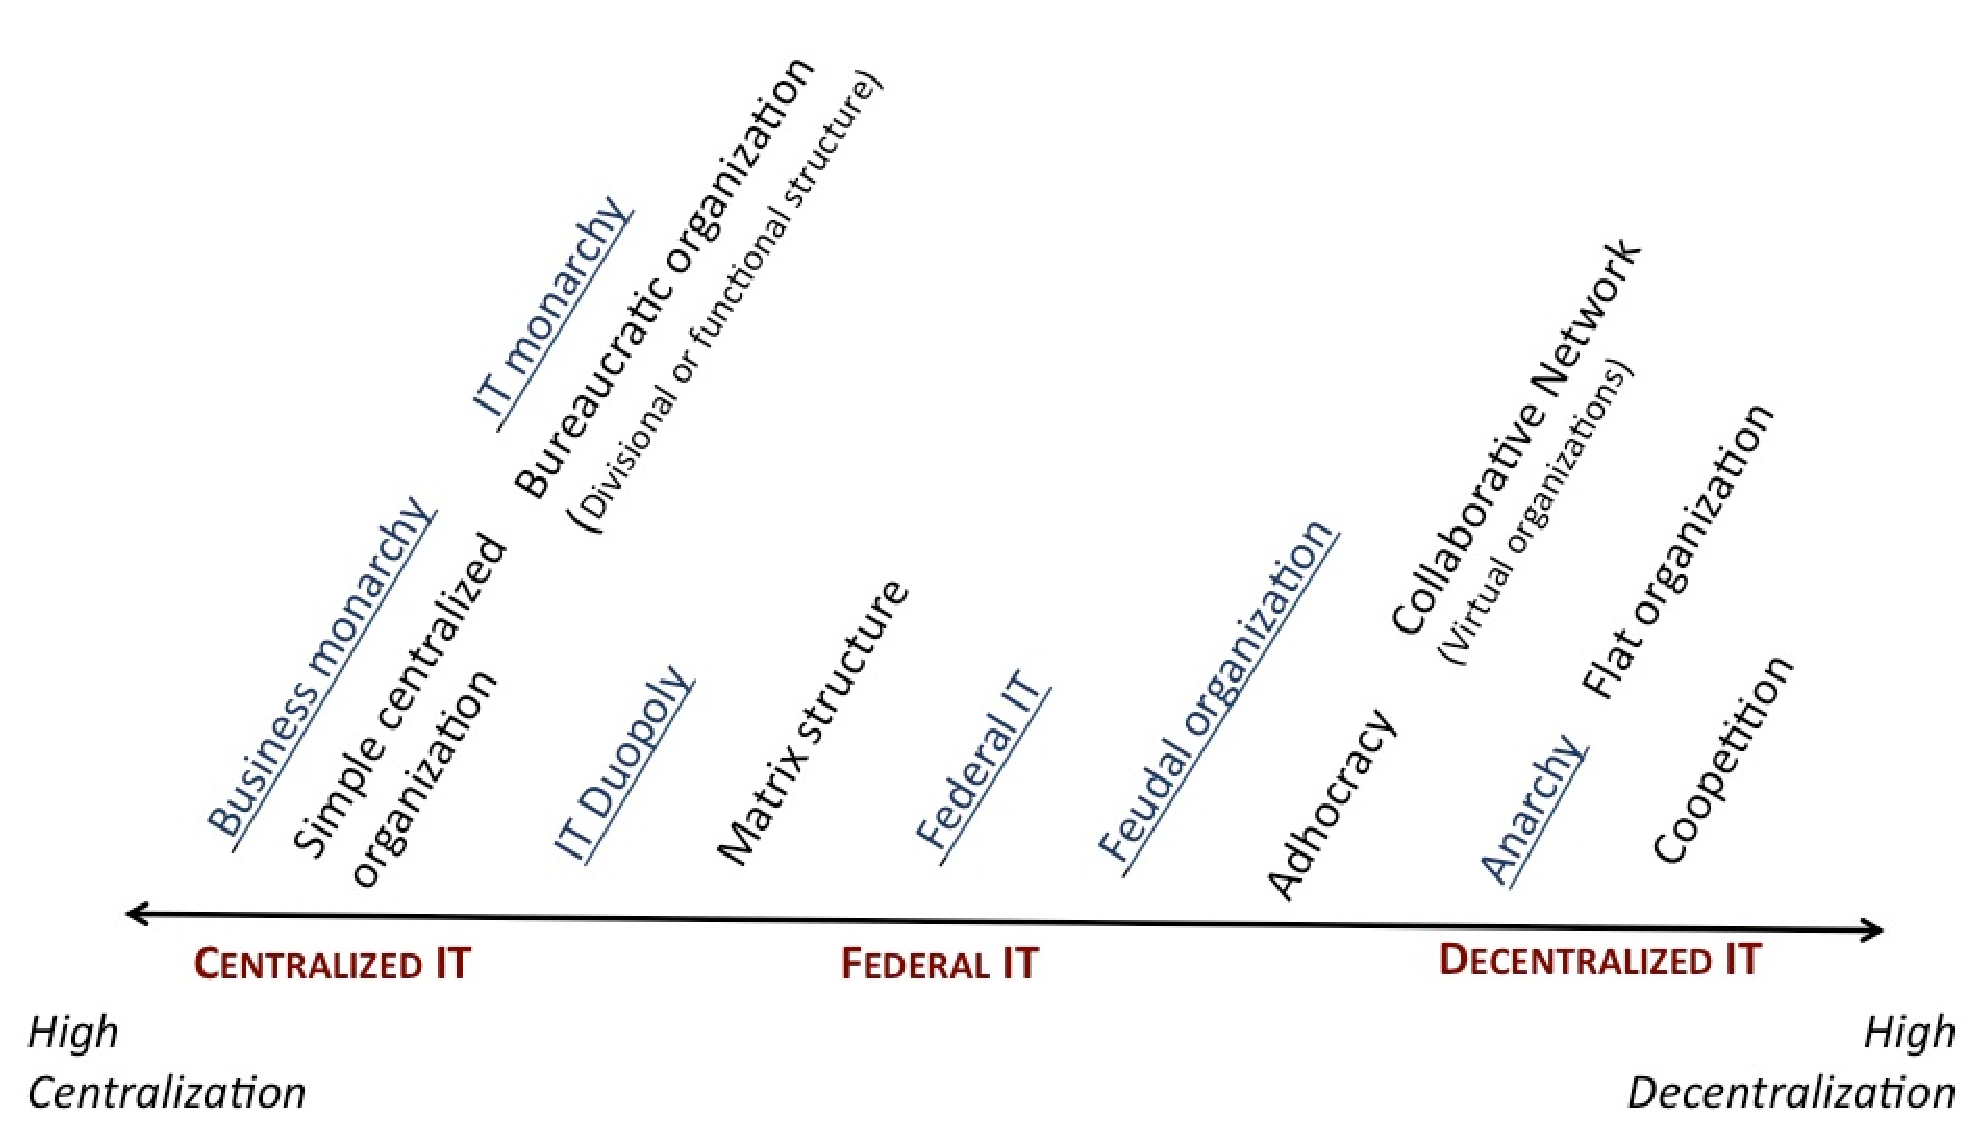
\includegraphics[scale=0.3]{taxonomy}
%\caption{Organizational taxonomy: From Centralized to Decentralized}
%\label{fig:taxonomy}
%\end{figure}

\subsection{Challenges of Progressive Decentralization in Organizational IT}
\label{sec:challenge}

%The trend appears to be moving away from the paradigm within which organizations strive for mass production efficiencies, hierarchical organization, and bureaucratic structures that provide central control over activities divided into small parts. The new paradigms may have as their premise the needed for flexible, learning organizations that continuously change and solve problems through interconnected coordinated self-organizing processes.

%From: Daft, Richard L., and Arie Y. Lewin. "Where are the theories for the" new" organizational forms? An editorial essay." Organization Science 4.4 (1993): i-vi.

%********

Modern organizational structures show a strong tendency towards decentralization \cite{daft1993} which results in changes to their management and operation styles. This heavily involves IT and requires major changes in organization processes. This transformation is not a mere question of ``flattening'' the organization by shifting authorities and decision making power from top to bottom hierarchical levels or from one person to a group. In classic organizations, not only does hierarchy ensure control and coordination, it also manages interdependencies between  different subunits of an organization which often makes direct interaction and communication unnecessary \cite{thompson1967}. As a result, a challenge related to decentralization and a ``weakened hierarchy'' is a lack of interaction and communication between organizational subunits. Another major risk of IT decentralization, according to \cite{Rockart1996}, is poor synergy and integration due to a lack of standardization.

Caruso, Rogers and Bazerman~\cite{caruso2008boundaries} highlight the importance of information sharing and coordination for these organizations. In order to succeed at these aspects, they outline three barriers that decentralized organizations need to overcome. The first barrier is intergroup bias; the tendency to treat one's own group better than other groups. The second barrier is group territoriality; the tendency for a group to protect their territory (physical or informational). The third barrier is poor negotiation strategies used by different groups when interacting with one another. 

Intergroup bias is direct result of having separate, autonomous groups within an enterprise~\cite{caruso2008boundaries}. The individual groups have a tendency to promote their own group over other groups, especially in situations where they are competing for a resource, such as a portion of the budget. A certain level of competition can be beneficial, however if it leads to hostility or distrust between groups, this can have a detrimental effect on their ability to share information and collaborate. This can prevent the groups from taking advantage of situations where they have to ability to work together for the benefit of everyone. 

The second barrier identified by Caruso et al. is group territoriality~\cite{caruso2008boundaries}. Group territoriality is characterized by group members taking action in order to protect their perceived territory. This can include physical territory such as space or tangible resources, as well as intangible territory, such as roles or information. Group territoriality is supported by a group's need to maintain its identity, its reputation of competence and sense of value, and a group's need for a stable home within the organization from which they interact with the rest of it. Group territoriality encourages ``a sense of psychological ownership''~\cite{caruso2008boundaries} for a group's members which can enforce the belief that they are the sole responsible party for a role or specific knowledge. This "inward-looking" behavior works against collaboration and information sharing. On the other hand, group territoriality can be beneficial; it can foster a sense of security in its members that ``facilitates planning and execution of activities''~\cite{caruso2008boundaries}. 

The third barrier identified by Caruso et al. in decentralized organizations is related to negotiations between groups, and how these negotiations are often conducted using ``poor negotiation  strategies''~\cite{caruso2008boundaries}. These poor strategies are the result of three common errors made while negotiating. The first error is a false belief in a ``fixed pie'' of value that is to be divided when negotiating. This prevents negotiating parties from recognizing situations where they are able to help each other, and therefore increase the size of the figurative pie. The second error is a failure to properly consider the other group's perspective. Understanding the other group's decision process, valuing process, and interests is key to discovering opportunities for helping one another, and the organization as a whole. The third error is when groups fail to even recognize they are in the process of negotiating. Instead, they see it as a competitive or hostile behavior where, again, they only see a fixed pie that is to be split up. This also prevents groups from taking advantage of opportunities to increase the size of the pie.    



   
    
    \section{Related Works}
    \label{sec:related}
    The practice of EA is just one potential solution to the problems of business-IT alignment. EA is a ``heavy-weight'' approach in that it aims to be a complete solution. However, other ``light-weight'' solutions do exist that focus on specific aspects of business-IT alignment and this section will briefly outline one of them: enterprise modeling.
  
%\subsection{Enterprise Modeling}

``Enterprise Modeling is the art of externalizing enterprise knowledge which adds value to the enterprise or needs to be shared. It consists in making models of the structure, behavior and organization of the enterprise''~\cite{Vernadat200215}. Through modeling, practitioners aim to better understand the current or future organization and function an enterprise. To this end, common enterprise categories of enterprise modeling include goal, process and value modeling. 

\paragraph*{Goal Modeling}

Goal modeling aims to describe the goals of an enterprise, their interrelations, means for achieving these goals, and additional factors that impact them. A specific example of a goal modeling technique is the Business Motivation Model (BMM)~\cite{bmm2010}. In BMM, means, ends and influencers of an organization are modeled and assessed. Here, the focus is on understanding what an organization wants to achieve (i.e. goals). The relationship between an organizations goals and its means is described, though the specifics of the means are not. 
%An EA, on the other hand, might use goal models, but if so, would use them as part of a bigger whole. This is in contrast with EA which takes a holistic approach in describing an entire enterprise, not only its goals.

\paragraph*{Process Modeling}

According to Roshen, ``[a] business process is a collection of related, structured activities or tasks that produces a specific product''~\cite{roshen2009soa}. Business processes are a complicated matter, and as such, process modeling is used to describe them in a detailed and accurate manner, in order to understand how an organization creates some output. Many different modeling languages exist, for example, Business Process Model and Notation (BPMN)~\cite{model2011notation}, Event-driven Process Chain (EPC)~\cite[Ch. 6]{scheer2005process}, and UML Activity Diagrams~\cite{uml241}. Processes can exist within an organization (intra-organizational) or they can interact with processes from other organizations (inter-organizational). According to Weske~\cite{weske2012business}, ``the primary focus of intra-organizational business processes is the streamlining of the internal processes by eliminating activities that do not provide value''. Inter-organizational processes, on the other hand, aim to specify and streamline interactions with other organizations. 

\paragraph*{Business Value Modeling}

Business value modeling depicts the exchange of value between entities. Examples of value modeling languages are e3 Value~\cite{Gordijn2001e3value} and REA~\cite{pavel2006model}. Business value modeling is used to understand what an organization does in order to create value. This allows it to be used as a starting point for the exploration of business ideas, design of processes, or development of systems~\cite{johannesson2011lecture}.

\paragraph*{Holistic Approaches}

A holistic approach to enterprise modeling can also be taken, where a combination of modeling techniques are used to represent an entire enterprise. The relationships between different models are specified, and a method for making the models may also exist. An example of a holistic modeling technique is Enterprise Knowledge Development (EKD)~\cite{stirna2007ten,bubenko2001user}, where an organization is modeled using six different models, each with a different focus. EKD also specifies a process for creating the models. A holistic approach to enterprise modeling such as EKD is similar to EA in that it specifies a process (similar to the EA method) and set of models that represent an enterprise (similar to EA description). However it is also quite different from EA in that it does cover how to transform those models into actual enterprise change.

%
%\subsection{Enterprise Integration}
%
%According to Vernadat, ``Enterprise Integration (EI) consists in breaking down organizational barriers to improve synergy within the enterprise so that business goals are achieved in a more productive and efficient way''~\cite{Vernadat200215}. To accomplish this, Vernadat states that EI relies ``free but controlled flow of information and knowledge, and the coordination of actions''. To this end, three general perspectives on EI exist: information-oriented, service-oriented, and process-oriented~\cite{zdravkovic2012}.
%
%Information-oriented integration is aimed at the integration of data. Two key components of information-oriented integration are standardizing how data is represented and enabling efficient access to it throughout an enterprise. Typical approaches to this are: data warehousing~\cite{kimball2006data}, where data from across the enterprise is consolidated to a single data warehouse in batches; data federation~\cite{haas2002data}, where a single system is used to query multiple data sources; and data replication~\cite{wiesmann2000database}, where data is copied between data sources at regular intervals. 
%
%Service-oriented integration is aimed the integration of functionality. The dominant architecture for service-oriented integration is Service-Oriented Architecture (SOA). Here, functionality is organized into services--worked performed by one application for another application--which have the characteristics of  reusability and composability~\cite{roshen2009soa}. These characteristics are important as they allow for services to be shared across and between enterprises (reusability), and for multiple services to be used together to create a new service (composability). 
%
%Process-oriented integration uses enterprise knowledge in conjunction with systems knowledge in order to integrate on the business process level~\cite{Vernadat200215}. Process-oriented integration builds on service-oriented integration in order to automate and order services for the production of some product. This can be done in both intra- and interorganization contexts, and is accomplished with the use of process models and systems dedicated to process management~\cite{dumas2005process}. A key advantage of process integration is that it provides a basis for communication between the IT and business sides of an enterprise~\cite{dumas2005process}.
    
    % Part 3 - Method    
    
    \chapter{Method}
    \label{chap:method}
    \section{Choice of Research Method}

Empirical research ``aims at describing, explaining and predicting the world''~\cite[Ch. 1]{johannessonPerjons2012}. In comparison, design research additionally wants to improve upon the world through the development of artifacts. This thesis project aims to improve EA by proposing an artifact that can extend the support of existing EA frameworks for decentralization. As a result, a design research approach, specifically design science, will be utilized. The remainder of this section seeks to further demonstrate the suitability of design science and outline the specific research strategies and methods chosen. 

\subsection{Design Science and its Relevance to this Thesis Work}

Design science is concerned with the development and application of \textit{artifacts} aimed at solving some practical problem~\cite{hevner2004,johannessonPerjons2012} in a manner that is of general interest~\cite[Ch. 1]{johannessonPerjons2012}. 

In order to be relevant, Design Science must exist in some context. Johannesson and Perjons~\cite[Ch. 1]{johannessonPerjons2012} define a generic context for design science in terms of people, practices and problems. A practice is a set of related activities performed regularly by people. In the performance of a practice, people encounter practical problems. Two general kinds of problems exist; one where the current state of affairs problematic and the desirable state is neutral, and a second where the current state is neutral and the desirable state is an improvement. The artifacts created through design science can be used by people to solve these practical problems. These concepts are easily related to this thesis work: Enterprise Architecture is a practice with a problem of the second type.  The current state of EA can be seen as being neutral; the problems outlined in this thesis are not necessarily ones that EA practitioners are concerned with.  However, this thesis argues that existing EA frameworks -- each of which can be seen as an artifact composed of smaller artifacts -- can be improved by increased support for decentralization through the development of artifacts addressing the issue of decentralization. 

According to Johannesson and Perjons~\cite[Ch. 1]{johannessonPerjons2012}, artifacts themselves have an ``inner construction'', exist in an environment, and have a function. The inner construction refers to the inner components of the artifact and the relations between them. The environment refers to the artifacts practice, the people using it, and anything else in its surroundings that have an effect on it. Lastly, the function of an artifact is the result of using it in its practice. This definition of an artifact also relates well to this thesis work: the inner construction of our artifact (an EA framework for decentralized organizations) can, at a high level, be seen as an EA method, EA description, and EA engine. The relations for these components are outlined in Figure~\ref{fig:EA_general}. The environment of our artifact includes the practice of EA and all affected components of the decentralized organization using it, such as involved stakeholders and implementers. The function of our artifact is, on a high level, to bring the benefits of traditional EA to decentralized organizations (e.g. business-IT alignment).

There exist four different types of artifacts: constructs, models, methods, and instantiations~\cite{hevner2004,johannessonPerjons2012}. Enterprise architecture is concerned with the first three of those types: constructs, models and methods. 

\textit{Constructs} are ways to describe some phenomenon. They give a common language for talking about something, but do not make any assertions about reality. For example, the EA description component of an EA framework provides a common taxonomy for the different parts of an organization covered by EA. 

\textit{Models} represent other objects. EA makes use of models, specifically descriptive and prescriptive models. Descriptive models are used to represent a current situation and its challenges, such the ``as-is'' architecture from the EA description. Prescriptive models represent potential future solutions, such as the ``to-be'' architecture, also from the EA description.

\textit{Methods} define ``guidelines and processes for how to solve problems and achieve goals''~\cite[Ch. 1]{johannessonPerjons2012}. The EA method and EA engine  are primarily methods, the former to construct the EA description, the latter to ensure its proper use throughout its lifecycle. 

This thesis work, being much smaller in scale than an entire EA framework, will focus on the creation of \textit{guidelines} (a method artifact type) for supporting decentralization in EA.

\subsection{A Design Science Method Framework}
\label{sec:framework}

Having established the relevance of design science to this thesis project, this thesis will therefore follow the framework for a design science method presented by Johannesson and Perjons in ~\cite[Ch. 4]{johannessonPerjons2012}. This method is composed of five activities with input-output relationships: Explicate Problem, Outline Artifact and Define Requirements, Design and Develop Artifact, and Evaluate Artifact. Each activity has an output which serves as an input to the next activity (e.g. an explicated problem is the input to the Outline Artifact and Define Requirements phase). These activities are carried out in an iterative manner, meaning that the practitioner will move back and forth between them as opposed to working in a sequential manner. 

The Explicate Problem activity is concerned with outlining the problem addressed by the research work in detail. To this end, the problem's significance needs to be clearly stated and its underlying causes can be possibly identified and analyzed. The output of this phase an explicated problem. 

The Outline Artifact and Define Requirements activity is where the explicated problem is transformed into the requirements for a solution to said problem. The output of this phase is the set of requirements for the artifact. 

The Design and Develop Artifact activity is where the artifact itself is built based on the requirements for the artifact. The output of this phase is the artifact itself.

The Demonstrate Artifact activity takes the developed artifact and implements it in either a real or illustrative case in order to demonstrate its viability. The output of this phase is the demonstrated artifact. 

The Evaluate Artifact activity is to demonstrate the artifact's fulfillment of the requirements and the degree to which it solves the problem. The output here is an evaluated artifact. 

\subsection{The Role of Research Strategies and Methods in this Design Science Framework}

Each of these activities can make use of controls and resources. Controls are the knowledge used to govern an activity~\cite[Ch. 4]{johannessonPerjons2012}, and  resources are the knowledge used as a basis for the activity. In this method for design science, controls are the research strategies and research methods used. A research strategy is the overall approach used to answer a research question~\cite[Ch. 3]{johannessonPerjons2012}, and research methods are the concrete methods used to generate and analyze data. 


\subsection{Choice of Research Strategy}

Alternative strategies exist for undertaking research in the field of design science. A number of common strategies will be briefly outlined in order to discuss their suitability for this thesis. 

Surveys aim to take a comprehensive look at something by gathering data from a large number of different sources. This data is then analyzed in some manner. Surveys offer a wide view~\cite{denscombe2010good,johannessonPerjons2012}, and as such, are not well suited for a depth view of something. This does not fit in with this project which takes an in-depth look at EA frameworks. 

Experiments employ a controlled and artificial environment in order to isolate a small number of specific factors to study them in detail. The effects of manipulating variables in the environment needs to be precisely measured~\cite{denscombe2010good}. This poses a problem for EA as organizations are highly complex entities where it would be exceptionally difficult to exert precise control and precisely measure the effects. For this reason, experiments are not a suitable strategy for this project. 

In action research, the researcher is an active participant in affecting the environment they are researching. Here, the research is done as part of the practice, as opposed to it being a separate activity~\cite{denscombe2010good}. This could be a highly effective strategy for this thesis topic as it would allow the researcher to experience the problems of decentralization first-hand. Furthermore, action research is a cyclical process, meaning the researcher could repeatedly try out different solutions and evaluate their effects in order to come to a good solution. This would allow for a researcher in a decentralized organization the flexibility to find a solution that works. Despite this fit to the thesis topic, the practical issue of finding a decentralized organization that is willing to go through this process is a significant one. As a result, action research is not used in this project. 

Ethnography is similar to action research in that the researcher becomes a member of the environment being researched. The difference lies in that they are there to integrate themselves into it, rather than affect change~\cite{denscombe2010good}. This could be an applicable research strategy for understanding problems from the perspective of stakeholders, however finding a decentralized organization with some sort of EA (or at least an interest in it) is quite the challenge in itself. Additionally, ethnography requires a large time investment in order to integrate adequately into the environment of study, which is not feasible for a Master's project. For these reasons, ethnography is not used in this project. 

Case studies take an in depth view of a single instance of the practice where the problem of interest exists. Case studies are ideal when ``a researcher wants to investigate an issue in depth and provide an explanation that can cope with the complexity and subtlety of real life situations''~\cite{denscombe2010good}. This project is interested in an in depth view of the problem of suitability of EA for decentralized organizations and decentralized organizations are real life entities that are highly complex. Furthermore, in contrast with ethnography and action research, conducting a single case study fits in well with the scope of a Master's project; it is not necessary for the subject organization to invest large amounts of resources into the project and time investment of a case study fits in with a short-term project. For these reasons, this thesis project will employ a case study research strategy.  

\subsection{Choice of Research Methods}

Research strategies do not prescribe any concrete ways to generate and analyze data. Specific research methods for data generation and data analysis are needed. 


\paragraph*{Data generation methods}

This thesis employs the use of interviews and document studies for data generation.  Document studies are used as a large amount of data on the structure of the organization being studied is available. Documents are a good source of authoritative, objective, and factual data~\cite{denscombe2010good}, which therefore gives a solid foundation on understanding the studied organization. Interviews were chosen in order to supplement this data with information from stakeholders about the organization. Interviews are suited for gaining insight into complex phenomena, which is supportive of our need for an in-depth view of a complex entity that is an organization. Furthermore, interviews are practical for this project as; a) the organization being studied does not need to invest large amounts of time and b) I have physical access to potential interviewees. 

Other common data generation methods are questionnaires and observations. Questionnaires are not particularly suitable for this project as they are most useful when used for specific, straightforward information~\cite{denscombe2010good}. This project, on the other hand, is interested in the complexities of an organization. An observation study would require spending time in an organization in order to directly observe its operations. As this thesis is conducted as an individual project, this is not a feasible activity, due to the size and complexity of an organization.

\paragraph*{Data analysis methods}

After the data has been obtained, it is necessary to analyze it in order to understand the object being studied. Data can be analyzed in either a quantitative or a qualitative manner. Quantitative data analysis is concerned with numeric data, whereas qualitative deals with words and visuals. According to Denscombe ~\cite{denscombe2010good}, some other differences between the approaches are; quantitative research is generally associated with large-scale studies whereas qualitative research is concerned with small-scale studies, and quantitative research is concerned with ``specific variables'' while qualitative research takes a ``holistic perspective''. This project follows a qualitative approach because; a) the data being analyzed will composed of words coming from interviews and document studies, b) this is a small-scale study, and c) this project is interested in a holistic perspective on our case study subject.

\section{Application of Method}

This thesis work follows the framework by Johannesson and Perjons~\cite[Ch. 4]{johannessonPerjons2012} presented above in Section \ref{sec:framework}. This section will first elaborate on how the different activities will be accomplished and then outline the overall process. 

As suggested in the framework, the IDEF0 notation will be used for visualizing the various activities. In this notation, each activity as an input and output, controls in the form of research strategies and methods, and resources which is the knowledge base for the activity.

\subsection{Case Study: An Institution of Higher Education in Sweden}
\label{sec:case}

This thesis work will use an institution of higher education in Sweden as an illustrative case study. This case was chosen as an example of a decentralized organization with an implicit EA, i.e., there is no formal EA framework used, but as they use IT extensively, some form of implicit architecture must exist. An advantage of this case is that, as a public institution, many official documents are available on its organizational structure, thus making a document study a viable research method. The documents that formed this study are described in Table~\ref{tab:doc_study}.

\textbf{MOTIVATION}

This thesis is not aiming at effecting change in this institution. The focus is instead on: analyzing the state of its EA in order to assess the decentralization support provided in contrast with what is needed; and proposing part of an EA that can provide the needed support. 

\begin{table}  
  \begin{tabular}[c]{| p{\dimexpr 0.4\textwidth-2\tabcolsep} |
                       p{\dimexpr 0.6\textwidth-2\tabcolsep} | }
    \hline
    \textbf{Document} & \textbf{Description} \\
    \hline
    Institution's homepage & Contains descriptions of the different organizational areas of the institution as well its organizational structure \\
    \hline
    Authority delegation documents & These publicly available documents specify authority and delegations of said authority of the institution's organizational units \\
    \hline
    Rule book & The official rule book of the institution detailing rules and decisions that must be followed by the institution \\
    \hline
  \end{tabular}
  \caption{Documents used in the document study}
  \label{tab:doc_study}
\end{table}

Four separate interviews are conducted in order to get a holistic view of the institution. The roles of the interviewees are: vice division lead, head of PhD studies, head of undergrad studies, and head of IT. The interviews are conducted in a semi-structured manner, starting with a set of open-ended questions that promote the interviewees to elaborate on their views. 

\subsection{Research Activities}
\label{subsection:research_activities}

\subsubsection*{Iterations Between Activities}

This research is conducted through two general iterations between the research activities:
\begin{description}
  \item[Iteration \#1] The first iteration focuses on using literature for conducting the research activities. In this iteration, the explicate problem activity, the generate sub-activity of design and develop artifact and a short demonstration were performed. %In this iteration, the activities explicate problem, outline artifact and define requirements, and the generate sub-activity of design and develop artifact were performed. 
  \item[Iteration \#2] The second iteration focuses on the case study in order to supplement the findings from the first iteration and to define the solution artifact. In this iteration, the activities explicate problem, outline artifact and define requirements, the search-and-select sub-activity of design and develop artifact, demonstrate artifact, and evaluate artifact were performed.%In this iteration, the activities explicate problem, outline artifact and define requirements, the search-and-select sub-activity of design and develop artifact, and demonstrate artifact were performed.
\end{description}

\subsubsection*{Explicate problem}

Figure \ref{fig:method_problem} outlines the major components of this activity:
\begin{description}
  \item[Sub-activities] Define Precisely, Motivate Problem and Find Root Causes~\cite[Ch. 5]{johannessonPerjons2012}
  \item[Input] The initial problem as described in Section \ref{sec:problem}
  \item[Resources] A literature study on centralization/decentralization in  organizational theory, and on the modern EA frameworks TOGAF, Zachman, and FEA. These three frameworks were chosen due to their popularity and extensive available literature.
  \item[Controls] A case study research strategy that will make use of interviews and a document study. The case is detailed in Section \ref{sec:case}. 
  \item[Output] A fully explicated problem, specifically, the set of specific shortcomings of modern EA frameworks when applied to decentralized organizations determined in the ``find root causes'' sub-activity.
\end{description}

\paragraph{Iteration \#1}

The first sub-activity, Define Precisely, is accomplished with the use of the literature reviews on centralization/decentralization in  organizations and on EA. A classification for decentralization organizations will be built from the literature review for use in the problem definition. 

In the second sub-activity, the problem is motivated through the use a literature review on decentralized organizations. Here, the differences between centralized and decentralized  organizations are specified in order to show that there is a problem. 

The third sub-activity, find root causes, is accomplished through a literature review. An in-depth analysis of each of the three EA frameworks will done to find specific shortcomings; aspects where the framework provides support for centralized organizations and not decentralized organizations. Aspects that are supportive of decentralization will be presented as well.

\paragraph{Iteration \#2}

In the first sub-activity, the problem in the case is precisely defined. In the second sub-activity, the problem is motivated through the use of the case study. To this end, a specific issue in the case that arises from their implicit EA and their organizational structure is identified.

The root causes of these issues are then determined in the third sub-activity. 

This is accomplished by identifying conflicts between the case organization's architecture principles, and its EA engine and supporting organizational structure.

\begin{figure}
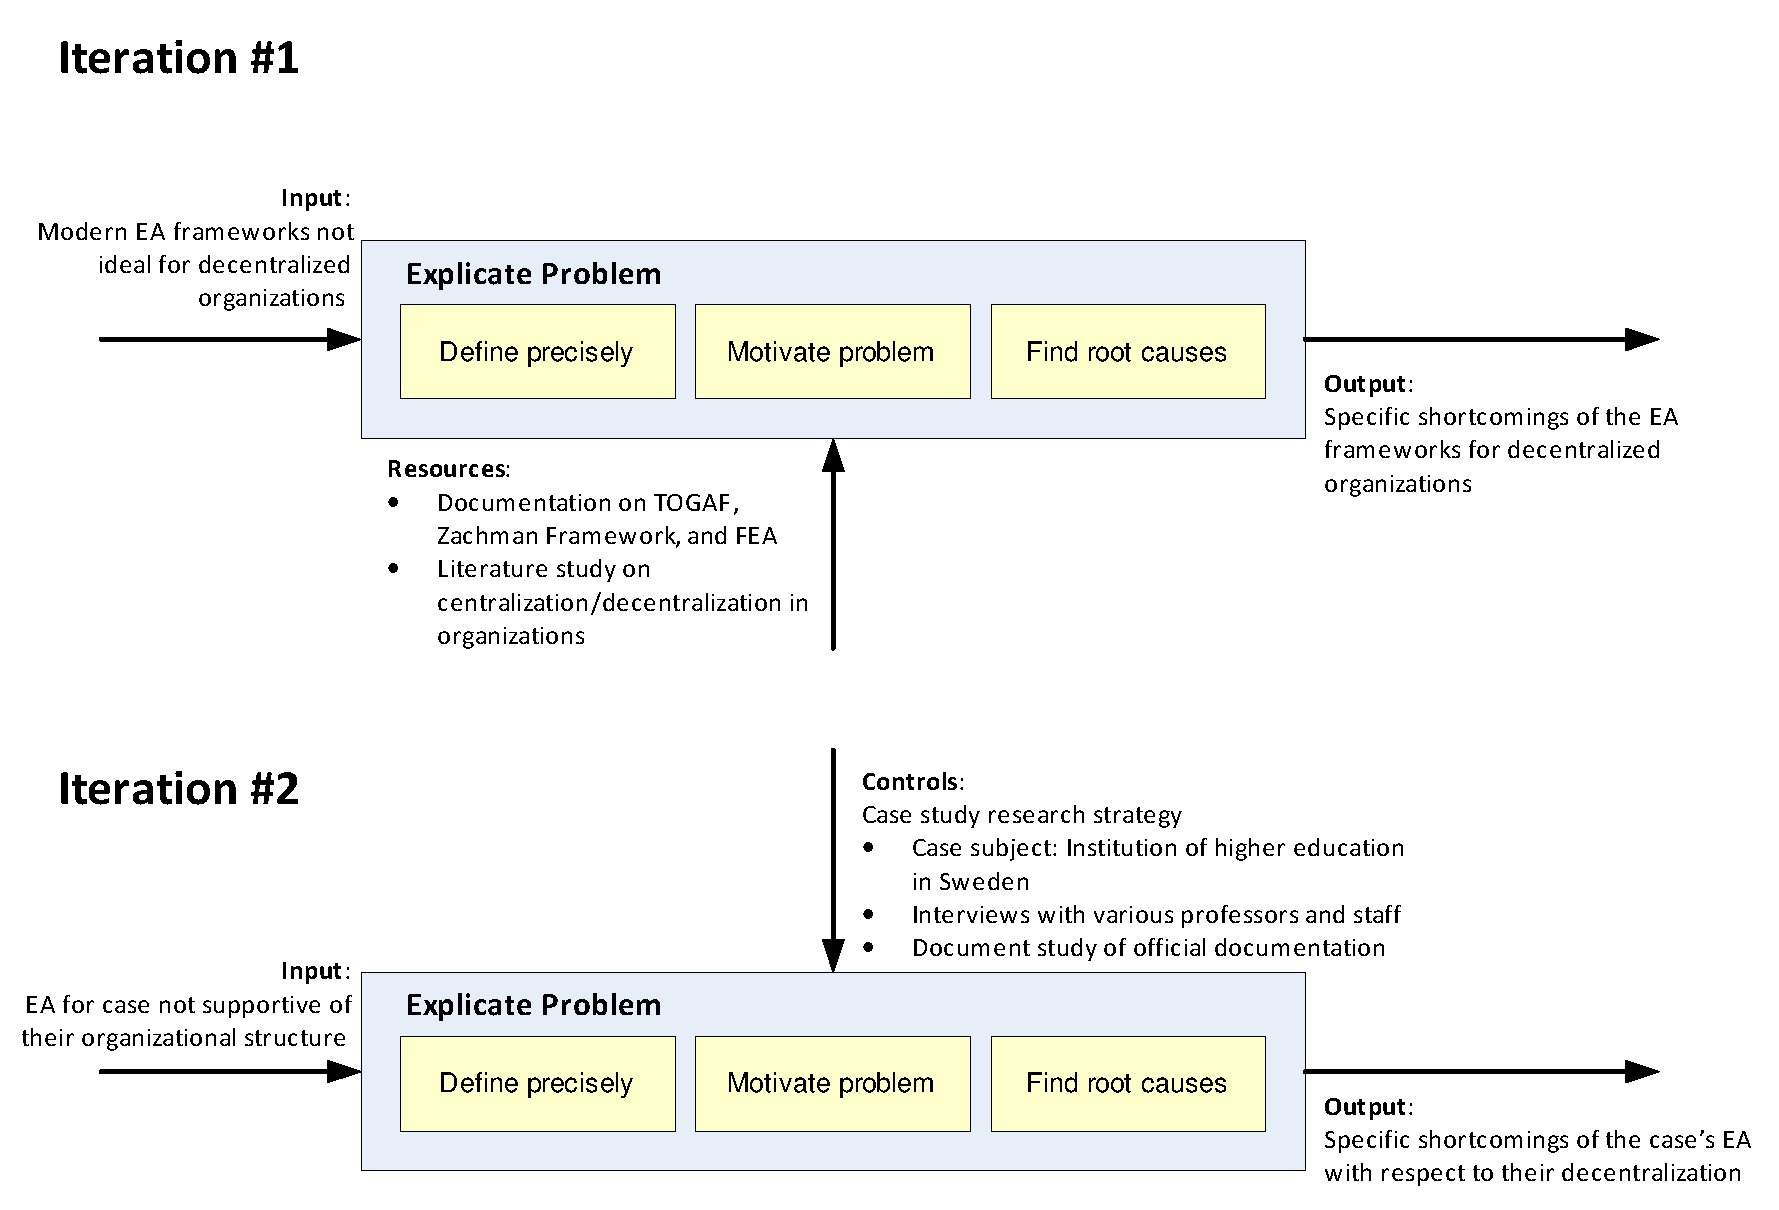
\includegraphics[scale=0.5]{method_problem}
\caption{Explicate problem activity}
\label{fig:method_problem}
\end{figure}

\subsubsection*{Outline artifact and define requirements}

Figure \ref{fig:method_outline} outlines the major components of this activity:
\begin{description}
  \item[Sub-activities] Outline Artifact and Define Requirements~\cite[Ch. 6]{johannessonPerjons2012}
  \item[Input] Set of specific shortcomings of modern EA frameworks when applied to decentralized organizations
  \item[Resources] Literature study on centralization/decentralization in  organizations
  \item[Controls] Case study research strategy
  \item[Output] An overview of the artifact and motivation for the selected artifact type (guidelines), and the requirements for the artifact
\end{description}

\paragraph{Iteration \#2}

In the first sub-activity Outline Artifact, the choice of artifact type, \textit{guidelines}, is explained and the artifact is described on a high level.

In the second sub-activity, Define Requirements, the requirements for the developed artifact are elicited. This is based on the specific shortcomings of the case's EA, the specific shortcomings of EA frameworks, and on the literature study on centralization/decentralization in organizations.


\begin{figure}
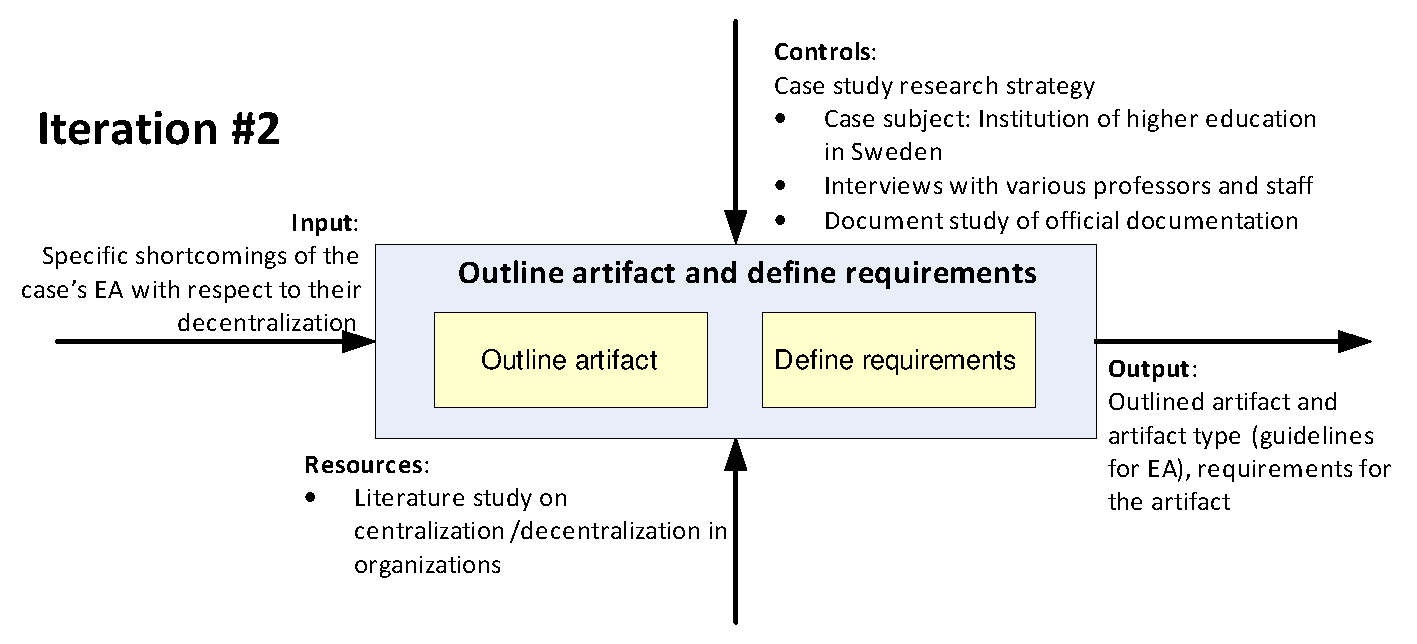
\includegraphics[scale=0.5]{method_outline}
\caption{Outline artifact and define requirements activity}
\label{fig:method_outline}
\end{figure}

\subsubsection*{Design and develop artifact}

Figure \ref{fig:method_design} outlines the major components of this activity:
\begin{description}
  \item[Sub-activities] Generate and Search and Select~\cite[Ch. 7]{johannessonPerjons2012}
  \item[Input]  Requirements for a decentralized EA 
  \item[Resources] Literature study on peer-to-peer architectures
  \item[Controls] None
  \item[Output] Prototype of one artifact for one aspect of an EA framework for decentralized organizations 
\end{description}

\paragraph{Iteration \#1}

In this iteration, only the Generate sub-activity is performed. Here, a small number of different peer-to-peer architecture principals that could potentially serve as solution artifacts are outlined using divergent thinking~\cite[Ch. 7.1]{johannessonPerjons2012}. The basis for these artifacts comes from a literature study on peer-to-peer architectures where principles relevant to EA are identified. Peer-to-peer architectures were chosen because they have offered solutions to decentralization in other domains (e.g. technical) and might therefore be able to provide solutions for the practice of EA.

\paragraph{Iteration \#2}

In this iteration, one of the outlined solutions is selected and elaborated on to create guidelines for EA in decentralized organizations. This selection is based on its applicability to the case, which is an example of a decentralized organization. 

\begin{figure}
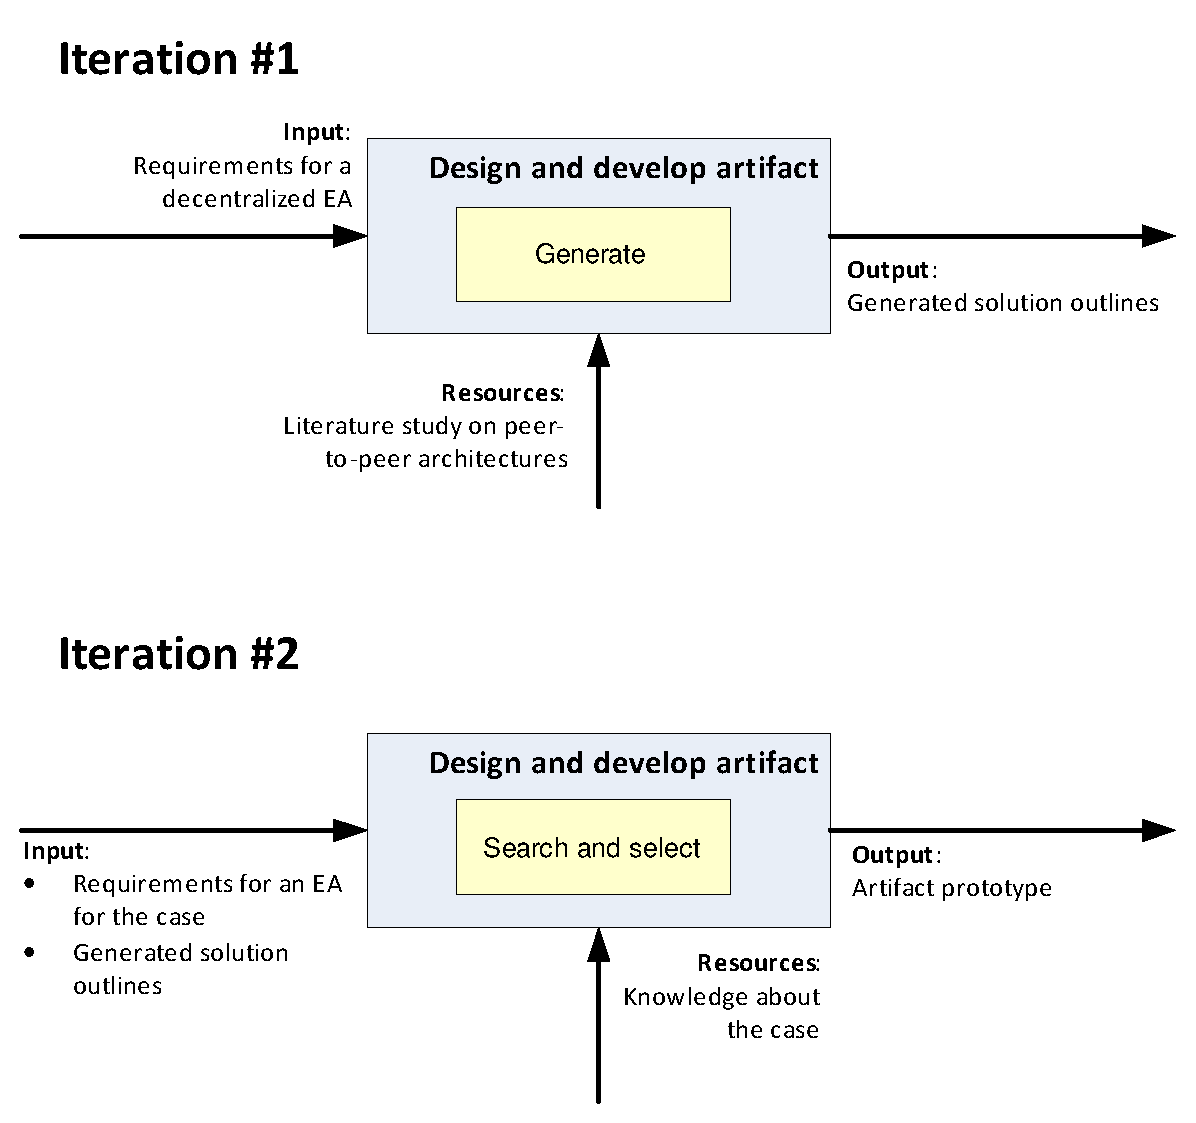
\includegraphics[scale=0.5]{method_design}
\caption{Design and develop artifact activity}
\label{fig:method_design}
\end{figure}
  
\subsubsection*{Demonstrate artifact}

Figure \ref{fig:method_demo} outlines the major components of this activity:
\begin{description}
  \item[Sub-activities]  Choose or Design Case and Apply Artifact~\cite[Ch. 8]{johannessonPerjons2012}
  \item[Input] Prototype of one artifact for one aspect of an EA framework for decentralized organizations; and feedback on the problem explication and potential solution outlines
  \item[Resources]  Knowledge on the selected case (institution of higher education in Sweden)
  \item[Controls]  A case study research strategy that will make use of interviews and a document study
  \item[Output] A demonstration of the solution artifact
\end{description}

\paragraph{Iteration \#1}

Here, the current state of the research (problem explication and potential solution outlines) is adapted to papers for submission to EA-related conferences. The output of this is feedback on the research.

\paragraph{Iteration \#2}
For the Choose or Design Case sub-activity, an institution of higher education in Sweden has been selected. Details on the case are described in \ref{sec:case}.

In the Apply Artifact sub-activity, three separate architectures are outlined: the As-Is architecture of the case, a To-Be architecture of the developed with the artifact, and a To-Be architecture based on traditional EA knowledge. These architectures will focus on one specific problem area of the case.

\begin{figure}
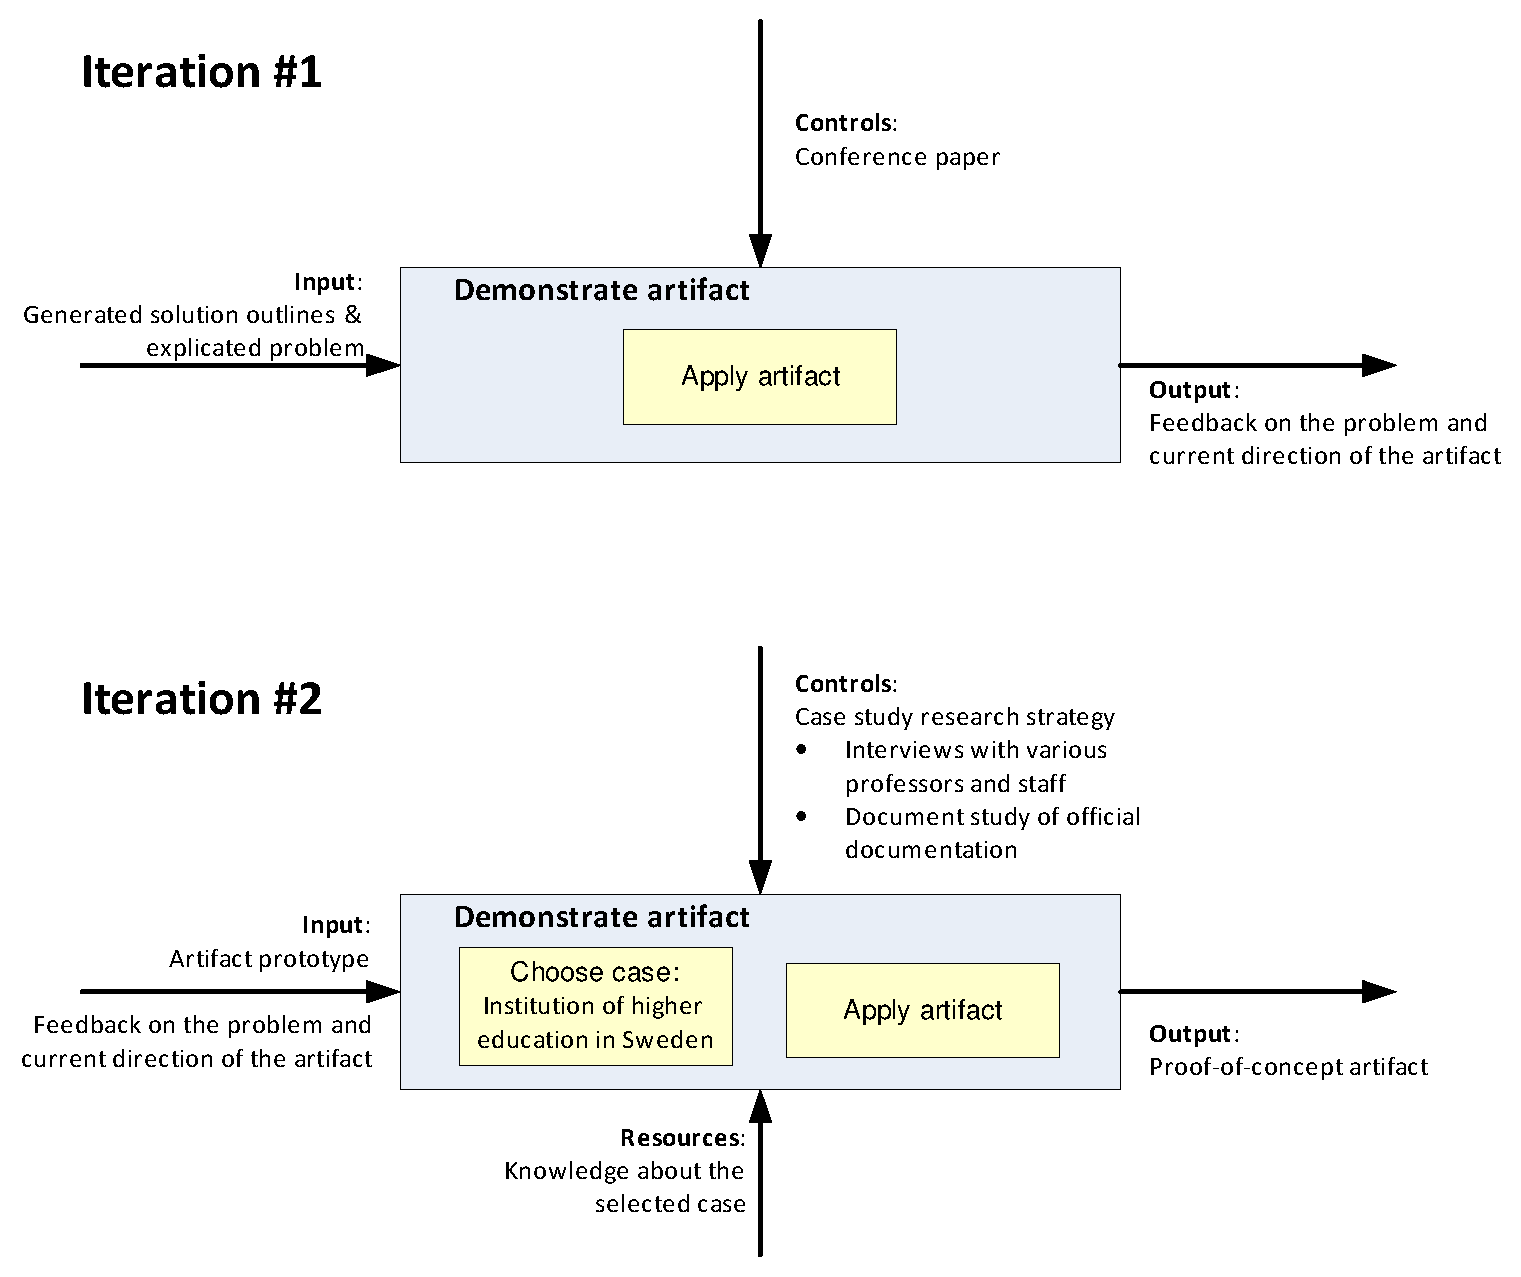
\includegraphics[scale=0.5]{method_demo}
\caption{Demonstrate artifact activity}
\label{fig:method_demo}
\end{figure}

\subsubsection*{Evaluate artifact}

Figure \ref{fig:method_eval} outlines the major components of this activity:
\begin{description}
  \item[Sub-activities] Choose Evaluation Strategy and Carry Out Evaluation~\cite[Ch. 8]{johannessonPerjons2012}
  \item[Input] Proof-of-concept artifact for one part of an EA framework prototype
  \item[Resources]  Knowledge on the selected case (institution of higher education in Sweden)
  \item[Output] An evaluated artifact
\end{description}

\paragraph{Iteration \#1}

This activity is not performed in the first iteration. 

\paragraph{Iteration \#2}

In the Choose Evaluation Strategy sub-activity, an \textit{ex ante} evaluation strategy is followed; this means that ``the artifact is evaluated without being used''~\cite[Ch. 9.1]{johannessonPerjons2012}. Johanneson and Perjons suggest interviews with experts for this sub-activity, however their are no experts available in the case organization, therefore an \textit{''informed argument``} approach is instead being followed. The chosen evaluation strategy must be able to show that the artifact solves the explicated problem and fulfils the defined requirements.

In the Carry Out Evaluation sub-activity, the decided upon evaluation strategy is carried out to create the output for this activity; an evaluated artifact. 

\begin{figure}
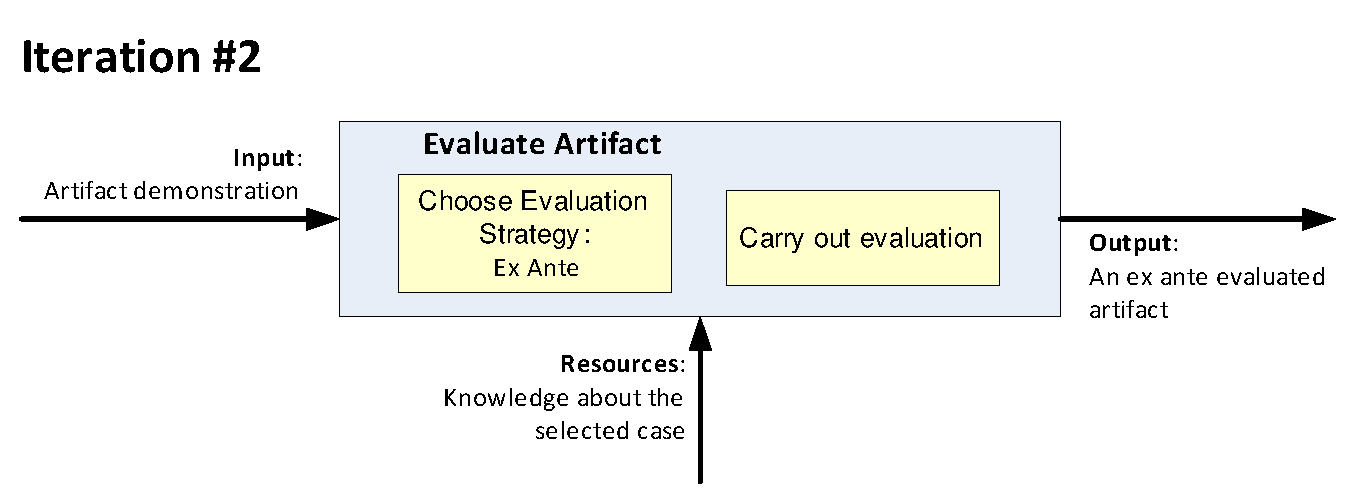
\includegraphics[scale=0.5]{method_evaluation}
\caption{Evaluate artifact activity}
\label{fig:method_eval}
\end{figure}

\label{sec:ethics}
\section{Ethical Considerations}

In any research project, the ethical conduct of the researcher is critical to not only the validity of the project, but to the research area a whole. As stated by Denscombe~\cite{denscombe2010good}: ``this expectation stems from the belief that the public should be protected from researchers who might be tempted to use any means available to advance the state of knowledge on a given topic.'' In this thesis, this is primarily applicable in two areas:

First, it is critical that I, as the researcher, do not let my personal beliefs on the current state of decentralization support in EA effect the collection, interpretation and analysis of the results of this thesis. In practice, it is not possible to completely remove all bias, but it is key that I maintain as neutral of a position as possible. For this reason, it is important that this thesis work identifies areas where EA supports decentralization, and not only areas where support is lacking. 

The second area where ethics were critical were in my interactions with the case organization. While no implementation was performed, it was still important that the wishes of the case organization are respected. Their wish is that they remain anonymous, and for this reason, their identity has been withheld from being published. Secondly, interviews are used as a means of data collection, and therefore, it is important that the beliefs of the interviewers are not pushed upon the interviewees. To avoid this, the interviewers will only guide the direction of the interview by asking questions, but will not provide any feedback about how they feel about the responses. 

    
    %Part 4 - Results
    
    \chapter{Results}
    \label{chap:results}  
    
    \section{Explicate Problem}    
    \label{sec:problem}
    %\subsection{Iteration 1}

\subsubsection{Define Precisely}

\paragraph*{Classification of Organizational Structures}

To precisely define our problem, we first need to define a taxonomy of organizational structures in order give a common way of describing these structures. To this end, we agree with Rockart, Earl and Ross~\cite{Rockart1996} who describe a continuum of IT governance styles ranging from centralized to decentralized, with federalism in the middle. Many organizations today tend to combine both centralization and decentralization in order to obtain the advantages of both styles: global integration and efficiency due to centralized management in some key areas and agility and high quality of local customer services due to decentralized decision making in others. 

For the purpose of this thesis work, three types of organizational structure in IT are considered along a centralization continuum: \textit{Centralized IT}, where all IT related decisions are made in a centralized manner by the top-level executives, \textit{Decentralized IT}, where each organizational subunit manages its IT in completely autonomous and independent manner,  and \textit{Federal IT} that can be seen as a combination of central IT management and IT management in the subunits. Here a primary task  would be to maintain standards for the entire enterprise while supporting flexibility on the subunit level. The business units would still have ownership of many of their own systems, allowing them to implement them as they deem best. 

Figure \ref{fig:taxonomy} maps the organizational forms presented in Section \ref{sec:organizations} to the continuum, ranging them from highly centralized (e.g. bureaucratic) to decentralized (e.g. virtual organizations).

\begin{figure}
\centering
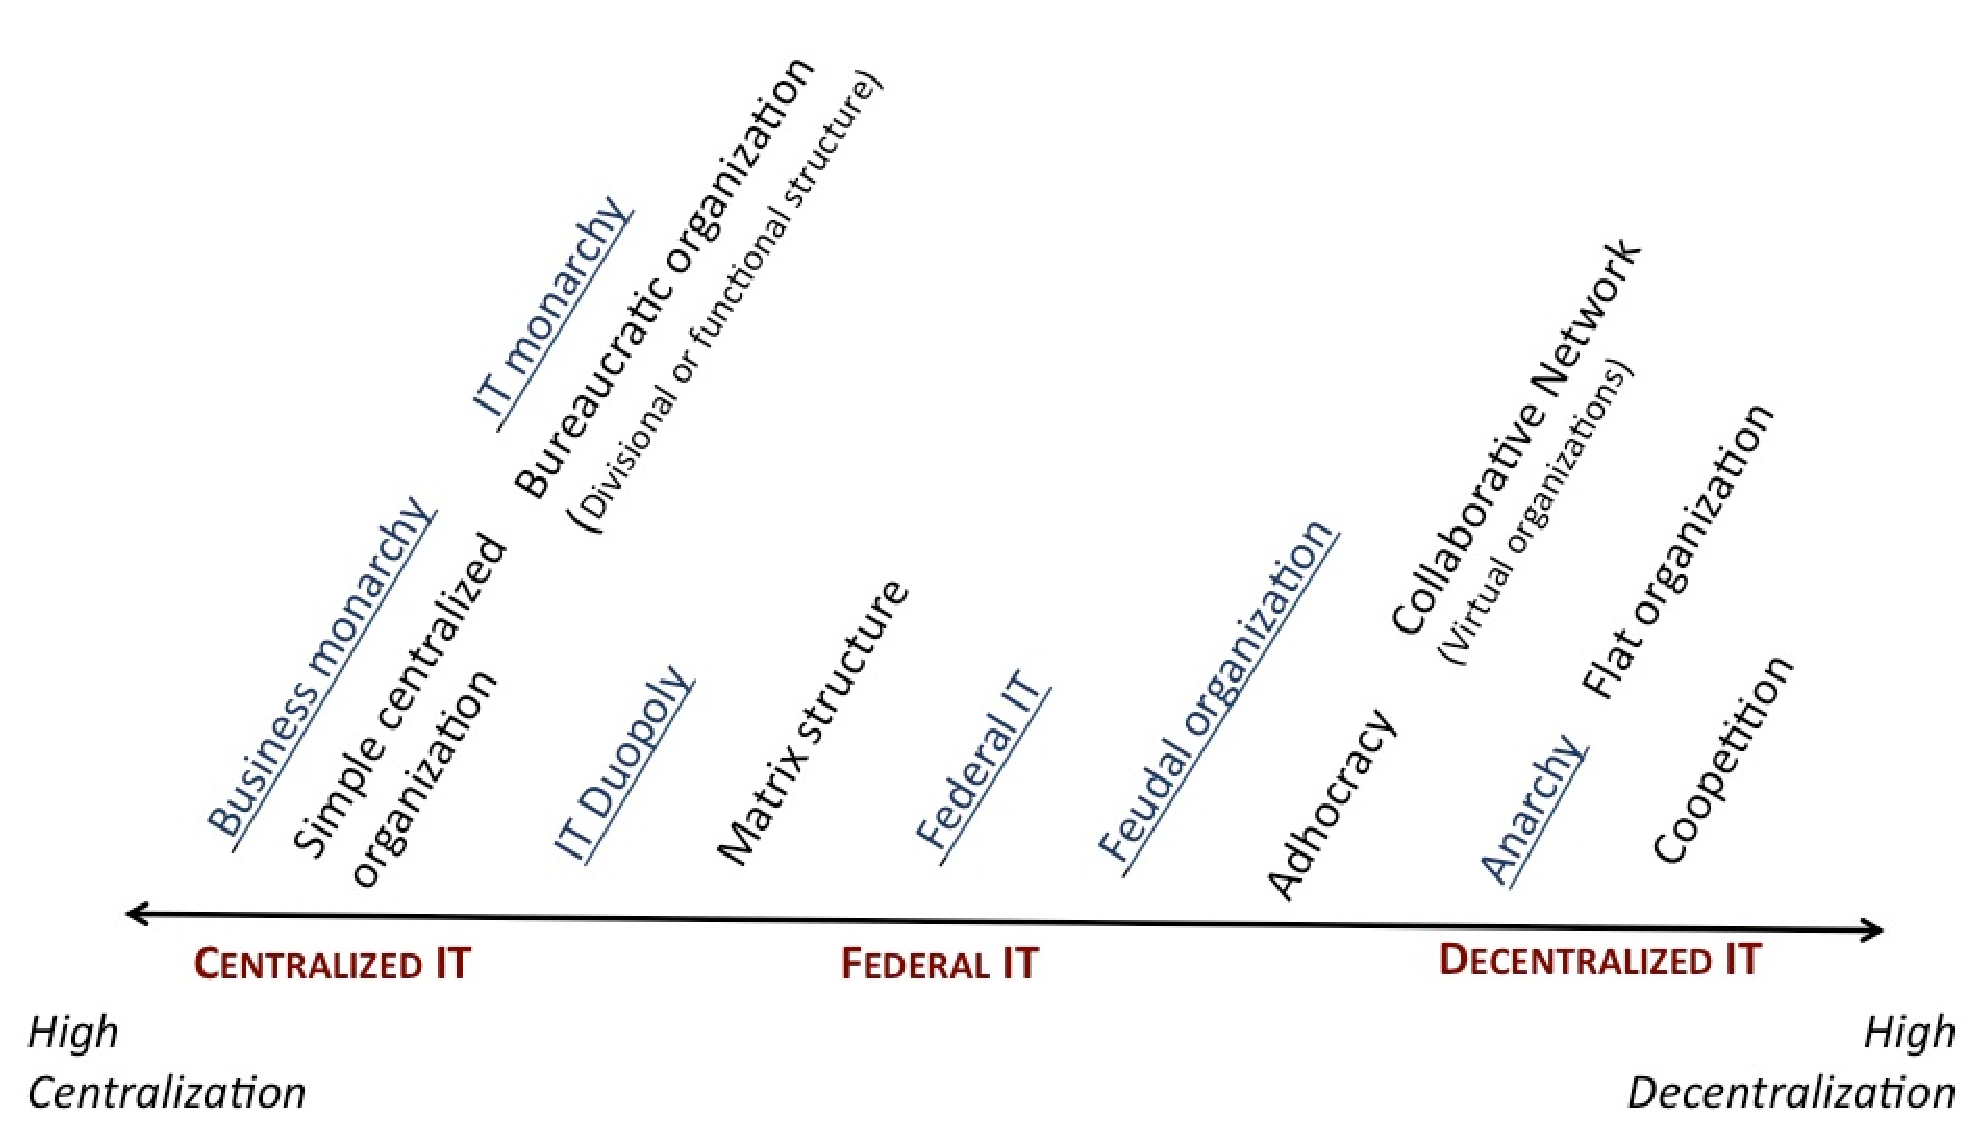
\includegraphics[scale=0.3]{taxonomy}
\caption{Organizational taxonomy: A Continuum From Centralized to Decentralized}
\label{fig:taxonomy}
\end{figure}

%TODO reflect in method

\paragraph*{Role of EA}

As detailed in Section \ref{sec:ea}, Enterprise Architecture is a discipline that allows an organization to construct and evolve its IT according to its needs. It provides a methodology and sets up a framework for assessing the current state of IT (architecture As-Is), for agreeing upon and communicating its future state (architecture To-Be), for planning, and for carrying out this transformation. By providing this framework, the modern EA frameworks of TOGAF, Zachman and FEA aim to solve the problem of business-IT alignment from the ground up through proper design. 

\paragraph*{The Problem} 

The EA frameworks of TOGAF, Zachman and FEA are primarily supportive of organizations with an structural form on the High Centralization end of the centralization continuum (Figure \ref{fig:taxonomy} ). This is a problem for organizations on the High Decentralization end of the spectrum, who will likely encounter issues if they implement EA as it is currently described in TOGAF, Zachman, and FEA. 


% **********************************************************************
% **********************************************************************
% **********************************************************************

\subsubsection{Motivate problem} %WHY PROBLEM IN IMPORTANT/RELEVANT
%TODO reflect in method

The problem of EA frameworks not being ideally suited for organizations on the High Decentralization end of the spectrum is important because: 1) organizations are becoming increasingly decentralized, and 2) EA can be beneficial to decentralized organizations. 

Organizations on the High Centralization end of the continuum fail to adapt to dynamic environments due to their inertia in decision making and lack of agility. As a result, organizations are moving more towards the High Decentralization, with organizational structures such as Flat and Collaborative Networks, where organizational subunits and individuals are being given an increasing amount of autonomy and control. THIS IS SUPPORTED HERE AND HERE AND HERE AND HERE AND HERE AND HERE. These structures support transparent or dynamically changing boundaries, agile processes, interactions aligned in real-time with changing business goals, virtual collaborations; all of which are technology-enabled capabilities.

Decentralization transforms the role of company's authority and makes relationships inside and between different company's divisions much more complex. Planning and governance in different functional areas, including IT,  is no longer centrally ensured. As a consequence, collaboration and information sharing between subunits gain extreme importance. This is evident in the challenges of decentralized organizations outlined in~\cite{caruso2008boundaries}. This is a significant change from the traditional management and operation styles of an organization and requires major changes in organizational processes. 

%TODO add more sources re: importance of communication/information sharing

While technology serves as an important catalyst for organizational transformations \cite{fulk1995,applegate1988}, it is important to utilize the right IT resources in a manner that is supportive of the organization. To accomplish this in decentralized organizations, novel EA processes, principles and concepts are needed to both handle the IT resources and to foster business/ICT co-evolution in decentralized environments. Consequently, changes to these EA frameworks in order to improve their support for decentralization would be beneficial for decentralized organizations. 



% **********************************************************************
% **********************************************************************
% **********************************************************************

\subsubsection{Find root causes}

The de-facto EA methodologies rely on organizational properties such as centralized management, global company identity, etc.  that are getting obsolete with progressive decentralization.  Consequently, implementation of these methodologies in decentralized organization becomes difficult and inefficient and  the role of EA as a driver for IT transformations is getting compromised.



\paragraph*{Key Differences Between Decentralized and Centralized Organizations}

Different organizational structures requires different EA...
 
Decentralized organizations face different challenges...

others:
Central: formal authority, standardization and rules in operations and in IT
Decentral:  Decentralized organizations lean towards lateral coordination characterized by meetings, task forces, coordinating roles, matrix structures, and networks [22].
Environment (stable vs unstable)
Control (more in top management in Centralized)
Division of labor
Conflicting goals
Communication lines
coopetition


\begin{table}
\caption{Cent vs Decent Characteristics}
\label{org_characteristics}
%%\begin{tabular}{l p{0.28\textwidth}}
\begin{tabular}{ | l | p{0.25\textwidth}| p{0.25\textwidth} |}
%
\hline
%
\textbf{Characteristic} & 
\textbf{Centralized} &
\textbf{Decentralized}  \\
%
\hline
%
Goals & 
Organization-wide goals set by upper management &
Frequently conflicting goals, but individual entities in the organization are working towards meeting common ones~\cite{Camarinha-Matos2005}
%
\hline
%
Geographical dispersion \cite{luthans2006} & 
Single location &
Geographically distributed with a reliance on IS to work together \cite{applegate1988} \\
%
\hline
%
Authority, decision rights and regulations & 
Decision rights are strictly defined and work their way down from the top \cite{Weill2004,pearlson2009}; strict governance and control by upper management \cite{pearlson2009,applegate1988}; rigid structuring of accountability and responsibilities \cite{applegate1988}; standard methods and procedures \cite{mintzberg1981} &
Authority and decision-making rights are pushed down to the level of groups, units or even individuals \cite{Weill2004,pearlson2009,robbins1997,Camarinha-Matos2005}; individuals can define their own roles and responsibilities \cite{valveHandbook} \\
%
\hline
%
Communication patterns \cite{thompson1967,pearlson2009,applegate1988} & 
hierarchy manages the interdependencies between the different sub-units of organization and often makes direct interactions and communications unnecessary \cite{thompson1967} 
communication lines are strictly defined and work their way down from the top.~\cite{pearlson2009} 
rigidly structuring "communication, responsibility, and accountability to help reduce complexity and provide  stability"~\cite{applegate1988} &
less formalized communication lines~\cite{pearlson2009}, and more fluid, project oriented teams.~\cite{applegate1988} \\
%
\hline
%
\end{tabular}
\end{table}








%Such organization structures are
%grounded on a sustainable collaboration between partners
%without any centralized control.

%collaborative
%networks (CN). Camarinha-Matos and Afsarmanesh
%define collaborative networks as being composed of ”a variety
%of entities (e.g., organizations and people) that are largely
%autonomous, geographically distributed, and heterogeneous
%in terms of their: operating environment, culture, social
%capital, and goals.” [24] Three common characteristics in
%various CNs are autonomy in the individual entities, a drive
%towards meeting common or complementing goals, and the
%use of an agreed-upon framework for collaboration.


%According to Robbins [18], organizational structure has
%three components: complexity, formalization and centralization.
%Complexity refers to the degree to which activities
%within the organization are differentiated; Formalization
%refers to the degree to which work is standardized; Centralization
%refers to the degree to which decision making is
%concentrated at one point in the organization.

%geographical
%or territorial concentration or dispersion of operations,
%functions, extent of concentration or delegation of decision
%making powers.


\paragraph*{TOGAF: Concepts supporting centralized organizations}

\subparagraph*{EA Method and EA Engine}
TOGAF outlines a formal approach to architecture governance which involves the setting up of an Architecture Board ``to oversee the implementation of the [architecture] strategy''~\cite[Ch. 47]{togaf9.1}. This board has an important role in Architecture Governance, such as ``[p]roviding the basis for all decision-making with regard to the architectures''~\cite[Ch. 47]{togaf9.1} and enforcing architecture compliance. 

%The TOGAF Architecture Governance Framework suggests guidelines for developing a formal governance structure for the Enterprise Continuum (and thus, all the architectural artifacts) and architecture processes. 

Architecture board concept suits well for the organization with strong centralization in IT (Centralized IT to Federal IT in Fig. \ref{fig:taxonomy}.  Having a single entity responsible for high-level decision making fits in with the concept of a Centralized IT organization. TOGAF does suggest that the board has enterprise-wide representation~\cite[Ch. 47]{togaf9.1} which may support some level of decentralization, however it suggests the representation comes in the form of ``senior managers''; a concept primarily from traditional organization structures. 

Throughout TOGAF, references are made to the existence of a bureaucratic or hierarchical centralized structure in place: 

For example, an important part of the preliminary phase [REF] is to set up a \textit{formal governance framework} for all architectural material, a concept that is related to the rigid forms of traditional organizational structure. 

Another example: after the completion of ``Phase A: Architecture Vision'', TOGAF requires approval of the current vision of the architecture. This requirement of approval assumes the existence of someone with a higher level of decision-making authority to give approval. 

A third example is an entire set of architectures at the strategic level of the Architecture Landscape which is meant for the ``executive level''~\cite[Ch. 20]{togaf9.1}.

\subparagraph*{EA Description}
TOGAF suggests the development of architecture principles that ``...define the underlying general rules and guidelines for the use and deployment of all IT resources and assets across the enterprise''~\cite[Ch. 23]{togaf9.1}. Having a central set of principles that is to be applied to an entire organization supports centralization.

TOGAF includes the concept of an Architecture Repository, which is to hold the entirety of the Architecture Landscape in addition to other architecture-related information. The idea of a single place to store all information is highly supportive of centralization. 

\paragraph*{TOGAF: Concepts supporting decentralized organizations}
\subparagraph*{EA Method and EA Engine}
TOGAF primarily supports some level of decentralization through the concept of \textit{partitions}. It suggests dividing the Architecture Landscape into separate parts in order to support multiple architecture teams working concurrently and conflicting architectures in different organizational units. This enables ``federated architectures — independently developed, maintained, and managed architectures that are subsequently integrated within an integration framework''~\cite[Ch. 40.3]{togaf9.1}. 

Furthermore, ``[f]ederated architectures typically are used in governments and conglomerates, where the separate organizational units need separate architectures''~\cite[Ch. 40.3]{togaf9.1}. This supports the idea of different organizational units developing their own individual architectures. The mechanism for integrating the individual architectures under the roof of the corporate architecture is not explicit. 


TOGAF additionally indirectly supports decentralization through the suggestion that the entire TOGAF process be\textit{ tailored to fit the needs of the enterprise}. This is done in the preliminary phase of the ADM. In theory, this would allow TOGAF to support any kind of enterprise. The guidelines provided for this, however, are minimal. 

\paragraph*{Zachman: Concepts supporting centralized organizations}
%Limited perspectives?
\subparagraph*{EA Description}
The Zachman Framework aims to model a complete enterprise in a single, ``periodic table of elements''~\cite{Bente2012}. It attempts to break down an enterprise into a matrix of 36 elements, with alignment and composite integration relations defined between these elements. 

The perspectives of Zachman Framework line up with a bureaucratic organizational structure: the defined views (from executive to user) constitute an explicit organizational hierarchy. Clear separation between domains make this framework suitable for matrix organizations as well. 
%(e.g. executive and business management perspectives).

The lack of flexibility in definition of domains and views and the requirement to fill in the matrix - is perhaps the Zachman Frameworks main shortcoming with respect to decentralization. A primary aspect of decentralized organizations is their high level of flexibility. For a decentralized organization where both roles and domains are not uniformly defined (implicit) for sub-units, the use of the Zachman Framework becomes difficult if at all possible.

%Furthermore, the perspectives of Zachman Framework line up with a bureaucratic organizational structure (e.g. executive and business management perspectives). For a traditional, centralized organization these perspectives make a lot of sense. 

\subparagraph*{EA Method and EA Engine}

Providing a schema for organizing architectural artifacts of an enterprise, the Zachman Framework does not imply any particular method for collecting these artifacts (what we call EA Method in Fig. \ref{fig:EA_general} ).
Neither is suggests the set of structures that we call EA Engine. 

Therefore, tailoring and  implementation of Zachman framework for a concrete organizational structure depends on experience of the EA (consultancy) team.

To summarize, the Zachman Framework provides a detailed taxonomy of EA artifacts that supports a hierarchical view on the organization. The application of this framework in decentralized (flat, adhocracy) organizations remains unclear.

\paragraph*{FEA: Concepts supporting centralized organizations}
\subparagraph*{EA Description}
Through the use of a common set of \textit{reference models}, FEA prescribes standards that are to be followed throughout the organization. This limits the flexibility that the individual organizational units have and makes this framework suitable for bureaucratic organizations with a high level of standardization of its processes.

In FEA, however, individual organizational units have the freedom to develop their own architecture as long as it fits in to the set standards. This supports some level of decentralization and suits to organizations with federal structure, where individual units have input into decisions. 

\subparagraph*{EA Method and EA Engine}

Segment architecture development is defined by FEA as a collaborative approach conducted by an integrated project team (IPT) comprising business subject matter experts, enterprise architects and technical subject matter experts.  FEA defines a set of segment architecture stakeholders and their roles (Table 2-2 in the document \cite{FEA_PMO2007} ) in segment architecture development.   For example, the role of senior management is defined to set the agency strategic goals; chief architect and EA team are appointed to supervise the architecture development process, coordinate the activities of other stakeholders and communicate and share the information between segments when needed; IPT activities and meetings are coordinated and managed by a Program Manager. The Program Manager should monitor progress, evaluate segment architecture completion and demonstrate results. These roles naturally line up with the centralized to federal organization of IT (Fig.\ref{fig:taxonomy} ).

According to FEA, ``Stakeholder commitment must be attained to support each step in this [development] process..''~\cite{FEA_PMO2007}.
 
The mechanism for integrating the segment architectures under the roof of the corporate architecture is  assured by specific governance and management processes, which are, tough implying different stakeholders, remain centralized. 

All steps of segment architecture development (Fig. \ref{fig:FEA_segmentDev} ) involve/supervised by the Program manager and/or chief architect or Capital Planning and Investment Control (CPIC) lead, pointing on centralized management and budgeting.

Transition strategy is defined for the agency level though it is assessed on the global level. Governance-wide collaboration and reuse based on standards is outlined by FEA as an important part of RA transition strategy.

\paragraph*{FEA: Concepts supporting decentralized organizations}
\subparagraph*{EA Description}

The resulting segment architecture is positioned by FEA as a shared vision for business and IT transformation within a core mission area or common service. Each segment can have its own architecture that responds to its business needs.

\subparagraph*{EA Method and EA Engine}

The development of \textit{segment architectures} is described as a collaborative process between EA architects and other stakeholders. The accent is placed on the ``reconciliation'' of the segment architecture with an agency architecture and cross-agency initiative, emphasizing the importance of  cross-agency collaboration, common opportunities and initiatives.

Architectural analysis and architectural definition steps of segment architecture development (Fig. \ref{fig:FEA_segmentDev} ) involve business owners at the agency level who define business and information management requirements for the segment. This allows to ensure the local, agency-level interests within a corporation. 

FEA is targeting the groups of independent federal agencies with an objective to increase their inter-operability and quality of service they are offering for citizens. Among three EA methodologies considered in our study, FEA is the only one recognizing the need of inter- and intra-agency cooperation and communication. Nevertheless, many of the concepts on which the EA method and EA engine of FEA are grounded remain strongly centralized. Again, this supports our initial claim.

\begin{table}
\caption{Existing and Prospective support of Progressive Decentralization by EA frameworks}
\label{summary}
%%\begin{tabular}{l p{0.28\textwidth}}
\begin{tabular}{ | l | p{0.25\textwidth}| p{0.25\textwidth} | p{0.25\textwidth}|}
%
\hline
%
EA component: & 
\textbf{Existing support for centralized organizations} &
\textbf{Existing support for decentralized organizations} &  
\textbf{Applicable P2P principles for a solution} \\
%
\hline
%
\textbf{EA Method:} & 
Approval process based on hierarchy; architecture development is coordinated, supervised and evaluated by well-defined roles in a company (e.g. senior managers define strategic goals); EA teams coordinate architectural work and communicate results; results are controlled and evaluated centrally - by program manager) &
Federated architectures; possibility to adapt ADM for a specific organization; architecture development process involves multiple stakeholders & 
peer production principles for creation and evaluation of EA artifacts; P2P trust management replacing approval mechanism\\
%flexible ADM & peer production; P2P trust management\\
%
\hline
%
\textbf{EA Description:} & 
Strategic level architectures; hierarchy of architecture principles; a common set of reference models; hierarchical organization of EA artifacts with explicitly defined roles and domains (Zachman) &
Architecture partitions; architecture reference models; segment architecture; the concept of ``shared vision'' & 
User-driven content submission and change management of the content (i.e. the structure is defined by the users)\\
%
\hline
%
%
\textbf{EA Engine:} &
Architecture board; formal governance framework; common set of principles for entire organization (i.e global commitment is taken for granted); centrally managed architecture repository &
integration of various (segment) architectures is assured by (centralized) management and governance &
Peer production for relevance/accreditation (e.g. decision making in budgeting, strategy, opportunity evaluation, solution evaluation); user-driven content submission and change management of the content; P2P trust management\\
%
\hline
%
\end{tabular}
\end{table}


% **********************************************************************
% **********************************************************************
% **********************************************************************


\subsection{Iteration 2}

\subsubsection*{Define Precisely}

DSV has decent/federated structure, needs supporting EA

% **********************************************************************
% **********************************************************************
% **********************************************************************

\subsubsection*{Motivate problem}

% **********************************************************************
% **********************************************************************
% **********************************************************************

\subsubsection*{Find root causes}

    
    \section{Outline Artifact and Define Requirements}
    \label{sec:outline}
    %%6.4 Guidelines for Outline Artefact and Define Requirements
%
%- Specify what artefact to build! Specify the artefact type (construct,
%model, method, instantiation) and its general characteristics.
%
%- Formulate each requirement clearly! Describe each requirement
%in a precise, concise and easily understandable way.
%
%- justify each requirement! For each requirement, explain why
%it is needed and relate it to the problem.
%
%- Be realistic but also original! Ensure that it is realistic to develop
%an artefact fulfilling the requirements but also try to be
%original.
%
%- Specify the sources of the requirements! Describe the literature
%and the stakeholders that have contributed to defining
%the requirements.
%
%- Describe how you have defined the requirements! Explain
%what you have done to define the requirements, in particular
%how you have reviewed the stakeholders and research literature.
%
%
%\subsection{Iteration 1}
%
%Not performed. 

%TODO Update method to match. Not doing 2 iterations here. Decide on which part of EA we do here. 
\subsection{Iteration 2}

\subsubsection*{Outline Artifact}

A key issue identified in the case is with decision making, where a mismatch exists between their integration- and centralization-focused architecture and an organizational structure with some highly decentralized aspects. This mismatch leads to problems in the ongoing success of the university's current architecture -- which is a problem addressed by the EA engine. Furthermore, as this issue lies in how decisions are made and enforced (i.e. the decision to have university-wide integration through use of a common system that cannot be enforced in practice), a governance framework which resolves these mismatches shall be developed. 

As identified in Section \ref{sec:exproblem}, an important property of a decentralized business environment that needs to be supported by EA is horizontal coordination. However, current EA frameworks primarily support vertical coordination in their governance styles, as identified in Section \ref{sec:exproblem} and Table \ref{table:summary}. Consequently, a different approach to EA governance is necessary for decentralized environments.

This thesis project will create an \textit{informal method artifact}~\cite[Ch. 2.4]{johannessonPerjons2012} in the form of a set of \textit{guidelines} to address this issue of governance in EA. These guidelines will be high-level Architecture Principles for a governance framework supporting decentralization.

%maybe not model, maybe something else

%For example, if IT systems
%need to be integrated to make a process more efficient, a solution
%can be a method for integrating IT systems, a model of an integration
%architecture, or an instantiation in the form of an integration tool.
%When the artefact type has been chosen, the artefact is to be described
%on an overview level.

%
%model or method
%
%However, models can also be used to describe
%potential solutions to practical problems, e.g. a drawing for a new
%type of vehicle or a proposal for an architecture of a mobile operating
%system. Such prescriptive models work as descriptions of possible
%future solutions and help to build artefacts that can solve practical
%problems.
%
%Methods express prescriptive knowledge by defining guidelines
%and processes for how to solve problems and achieve goals. In particular,
%they can prescribe how to create artefacts. Methods can be
%highly formalized like algorithms, but they can also be informal such
%as rules of thumb or best practices. Some examples are methods for
%database design, change management initiatives, or web service development.


\subsubsection*{Define Requirements}

The requirements for the artifact are outlined in Table \ref{table:requirements}.

\begin{table}
\caption{Requirements for the solution artifact}
\label{table:requirements}
%%\begin{tabular}{l p{0.28\textwidth}}
\begin{tabular}{ | p{0.5\textwidth} | p{0.5\textwidth} |}
%
\hline
%
\textbf{Requirement} & 
\textbf{Source}  \\
%
\hline
%
\textbf{1 The artifact shall support lateral coordination} & \\
%From Table \ref{table:org_characteristics} \\
%
%\hline
%
1.1 The artifact shall support decentralized authority structures & 
\cite{Weill2004,pearlson2009,robbins1997,Camarinha-Matos2005} \\
 %
%\hline
%
%1.2 The model shall support fluid roles &
%\cite{valveHandbook} \\
%
%\hline
%
1.3 The artifact shall support heterogeneous goals & 
\cite{Camarinha-Matos2005} \\
%
%\hline  
%
%The model shall support conflict resolution of conflicting goals  & 
%Implied from the previous requirement \\
%
\hline
%
\textbf{2 The artifact shall support governance activities}  & 
 \\


2.1 The artifact shall address architecture interoperability and integration issues &
The primary purpose of governance in FEA \cite[Sec. 2]{FEA_PMO2007} and TOGAF \cite[Ch. 50]{togaf9.1} is to ensure architecture components work well with one another for meeting an organization's goals \\

\hline
%
\end{tabular}
\end{table}

 
    
    
    \section{Design and Develop Artifact}
    \label{sec:design}
    %\subsection{Iteration 1}

\subsubsection*{Generate}

The challenge of decentralization is not a new one; other efforts have been able to address their view on it with success. The specifics of the challenge varies between domains, however there may exist general principles that can be taken and applied to EA. 

One such effort is peer-to-peer architecture. According to Saroiu, Gummadi and Gribble, peer-to-peer systems ``...typically lack dedicated, centralized infrastructure, but rather depend on the voluntary participation of peers to contribute resources out of which the infrastructure is constructed. Membership in a peer-to-peer system is ad-hoc and dynamic...''~\cite{saroiu2001measurement}. 

%Multiple parallels can be drawn between the problem decentralization for peer-to-peer systems and the problem of decentralization for EA.

We argue that peer-to-peer is a relevant concept to decentralization in EA for two reasons. First, individuals in highly decentralized organization are able to contribute to the enterprise in a manner that is completely up to them. This is similar to peers in a peer-to-peer system, where the peers participate in a completely voluntary manner. Second, the challenge that peer-to-peer systems overcome is similar to the main challenge faced by decentralized organizations. Saroiu et al. state that the challenge of peer-to-peer systems is to ``to figure out a mechanism and architecture for organizing the peers in such a way so that they can cooperate to provide a useful service to the community of users''~\cite{saroiu2001measurement}. This is similar to the main challenge facing decentralized organizations--a lack of interaction and communication, or in other words, cooperation--which was identified in Section \ref{sec:challenge}. 

With EA being a potential solution to this challenge of decentralization in organizations and the parallels between the domains of peer-to-peer systems and decentralized organizations, we propose that peer-to-peer may be a potential source of principles that could form the basis for evolving current centralization-focused EA frameworks into ones that are supportive of decentralization. This section outlines solutions based on relevant principles from peer-to-peer that have been generated through brainstorming.

%
% Theory: 
%

\paragraph*{Peer production}

Benkler defines peer production as ``...production systems that depend on individual action that is self-selected and decentralized, rather than hierarchically assigned''~\cite{benkler2006wealth}. Here, individuals act according to their own will rather than being directed by a central figure. Peer production works on the idea of the individuals willingly coordinating with one another by expressing their own views while understanding the views of others.

%
%% Examples:
%

Peer production takes many different forms. One example are user-driven media sites such as Reddit\footnote{~\url{www.reddit.com}} and Slashdot\footnote{~\url{www.slashdot.org}}, which follow a peer-production model for producing ``relevance/accreditation''~\cite{benkler2006wealth} on user-submitted content. On these sites, the users have the ability to vote on the submitted content in order to decide on the content's relevance or credibility. Another example of relevance production are crowdfunding sites such as Kickstarter\footnote{~\url{www.kickstarter.com}} where individuals decide on the funding of user-submitted projects by giving their own money. Peer production is also used to produce content, such as in the case of Wikipedia\footnote{~\url{www.wikipedia.org}}, an online encyclopedia which provides a platform for user-driven content submission and change management of that content.

%
%% Why Appropriate:
%

If we view enterprises as being composed of peers (a peer could be individual or an organizational unit), the idea of peer production becomes useful for EA. For example, the EA  Engine of TOGAF relies on an Architecture Board responsible high-level decisions and governance. Instead of a central board responsible for making decisions, a model based on the principle of peer production for relevance/accreditation could be used instead. This would better support decentralization as decision making would then be distributed amongst the peers that make the organization.

%%
%% Theory: 
%%

\paragraph*{Trust management in peer-to-peer}
%
%% Definition:
%
Due to the fact that peers in peer-to-peer systems are able to operate in a completely independent manner, there exists the problem of knowing whether or not the contribution made by a peer is trustworthy or not. Consequently, some researchers have proposed various methods for determining trust in a peer-to-peer environment.
%
%% Examples:
%
For example, Aberer and Despotovic~\cite{aberer2001managing} have proposed determining whether a peer is trustworthy or not based on a peers history of interactions with other peers in the system. This assessment is performed by the individual peers, and as such, is appropriate for a peer-to-peer environment.
%
%% Why Appropriate:
%
TOGAF employs the idea of an approval process grounded on the presence of centralized authority. This is to ensure that the presented architectural material is in fact valid for the enterprise. In a decentralized environment, this central authority is not likely to exist. Peer-to-peer trust management may offer a solution here. Instead of being give an explicit stamp of approval, the acceptance of a peer's contribution to EA by other peers can be based on a peer's level of trustworthiness. 
%
% 
%
%vice division lead \interview1{}, head of PhD studies \interview2{}, head of undergrad studies \interview3{}, and head of IT \interview4{}  
%...\footnote{Text to repeat\label{fn:repeat}}
%...
%...\footref{fn:repeat}

%one \footnote{From the interview with the division vice-lead\label{fn:interviewHead}}
%two \footnote{From the interview with the head of PhD studies\label{fn:interviewPHD}}
%three \footnote{From the interview with the head of undergrad studies\label{fn:interviewUndergrad}}
%four \footnote{From the interview with the head of IT\label{fn:interviewIT}}
%five \footnote{From the document study\label{fn:document}}
%one2 \footref{fn:interviewHead}
%two2 \footref{fn:interviewPHD}
%three2 \footref{fn:interviewUndergrad}
%four2 \footref{fn:interviewIT}


\subsection{Iteration 2}
\label{sec:design_iteration2}

\subsubsection*{Search and Select}
%EA Engine - ensure ongoing success of achitecture
%A key issue identified in the case is with decision making, where a mismatch exists between their integration- and centralization-focused architecture and an organizational structure with some highly decentralized aspects. This mismatch leads to problems in the ongoing success of the university's current architecture -- which is a problem addressed by the EA engine. Furthermore, as this issue lies in how decisions are made and enforced (i.e. the decision to have university-wide integration through use of a common system that cannot be enforced in practice), a governance framework which resolves these mismatches has been developed. 
%
%
As the problem outlined in ``Iteration 2'' Section~\ref{sec:exproblem} relates primarily to the decision making aspect of the university's EA engine, the principle of peer production will be used to form the basis of the solution artifact.  The principle of trust management in peer-to-peer would be useful in determining whether some produced content (i.e. an EA artifact) is of sufficient quality to be included in the overall architecture, but is not as applicable to the problem of a mismatch between decision-making structures. 

As highlighted in table~\ref{table:summary}, EA frameworks often assume vertical coordination, for example the Architecture Board of TOGAF. Here, some central authority is responsible for the overall decision making with respect to the architecture. This thesis instead instead proposes a peer production-based governance framework where this decision-making authority is instead distributed to whoever is affected by the outcome of the decision. The specifics of this heavily depend on the organization implementing it, but the following general guidelines are proposed:

\paragraph*{Willful coordination} Instead of strict, formal compliance measure, operate under the principle that the architecture requires willful coordination by individual entities. This is based on the idea from peer production that individuals willingly coordinate with one another for the purpose of mutual benefit.

\paragraph*{Decentralized authority structure} Allow for operational departments to make decisions for themselves about their relevant areas, thus granting them freedom to do as they see best. With respect to IT, for example, an individual business unit should have the authority to decide which systems they should develop themselves, and when they should collaborate with the rest of the organization. 

\paragraph*{Peer decision making} Decision making should be distributed to the affected individuals as opposed to residing with an top-level entity. This can be done by giving everyone the right to vote on a decision. Since it is however not feasible to vote on all decisions, such voting should be reserved more for major decisions. 

%
%
%
%
%
%
%
%
%
%
%
%
%
%
%
%%%%%%%%%%%%%%%%%%%%%%%%%%%%%%%%%%%%%%%%%%%%%%%%%%%%%%%%%%%%
%%%%%%%%%%%%%%%%%%%%%%%%%%%%%%%%%%%%%%%%%%%%%%%%%%%%%%%%%%%%
%%%%%%%%%%%%%%%%%%%%%%%%%%%%%%%%%%%%%%%%%%%%%%%%%%%%%%%%%%%%
%%%%%%%%%%%%%%%%%%%%%%%%%%%%%%%%%%%%%%%%%%%%%%%%%%%%%%%%%%%%
%Random notes
%
%
%%%Benkler defines peer production as ``...production systems that depend on individual action that is self-selected and decentralized, rather than hierarchically assigned''~\cite{benkler2006wealth}. Here, individuals act according to their own will rather than being directed by a central figure. Peer production works on the idea of the individuals willingly coordinating with one another by expressing their own views while understanding the views of others.
%%%
%%%%
%%%%% Examples:
%%%%
%%%
%%%Peer production takes many different forms. One example are user-driven media sites such as Reddit\footnote{~\url{www.reddit.com}} and Slashdot\footnote{~\url{www.slashdot.org}}, which follow a peer-production model for producing ``relevance/accreditation''~\cite{benkler2006wealth} on user-submitted content. On these sites, the users have the ability to vote on the submitted content in order to decide on the content's relevance or credibility. Another example of relevance production are crowdfunding sites such as Kickstarter\footnote{~\url{www.kickstarter.com}} where individuals decide on the funding of user-submitted projects by giving their own money. Peer production is also used to produce content, such as in the case of Wikipedia\footnote{~\url{www.wikipedia.org}}, an online encyclopedia which provides a platform for user-driven content submission and change management of that content.
%%%
%%%%
%%%%% Why Appropriate:
%%%%
%%%
%%%If we view enterprises as being composed of peers (a peer could be individual or an organizational unit), the idea of peer production becomes useful for EA. For example, the EA  Engine of TOGAF relies on an Architecture Board responsible high-level decisions and governance. Instead of a central board responsible for making decisions, a model based on the principle of peer production for relevance/accreditation could be used instead. This would better support decentralization as decision making would then be distributed amongst the peers that make the organization.
%
%
%TOGAF ACF
% - board (responsibilities include “[p]roviding the basis for all decision-making with regard to the architectures”,)
% - a formal architecture compliance process (to “[f]irst and foremost, catch errors in the project architecture early, and thereby reduce the cost and risk of changes required later in the lifecycle”)
% - the use of architecture contracts
% - guidelines for architecture governance
%
%
%FEA describes “EA governance and management processes” [4, Sec. 2] to control architecture development. These process are implemented to manage standards, enforce compliance, manage collaboration between agencies, approve architectures for implementation, and manage business and IS requirements for managing EA change.
%
%Segment architecture development is controlled by EA governance and management
%processes across each phase of the Performance Improvement Lifecycle. Governance
%and management processes are implemented to:
%• Review segment architecture work product content and format standards to
%promote reconciliation with the agency EA and relevant cross-agency initiatives;
%• Validate opportunities for agency-level and cross-agency collaboration and reuse
%including the implementation of relevant cross-agency initiatives;
%• Review and approve segment architecture in advance of IT investment and
%project execution;
%• Capture segment-level business and information management requirements to
%update and maintain the agency EA; and
%• Capture lessons learned to improve the segment architecture process and
%standard work products.
%
%- Clearly describe each component of the artefact! Describe both the functionality and construction of each artefact component.
%
%- Justify each component of the artefact! Explain the purpose of each artefact component, in particular which requirement(s) it addresses.
%
%- Describe the use of the artefact! Describe how the artefact and its components are intended to be used in its intended practice.
%
%- Clarify the originality! Describe in what respects the artefact is different from existing ones with respect to both functionality and construction.
%
%- Specify the sources of the artefact design! Describe the literature and the stakeholders that have contributed to components of the artefact and/ or inspired the design of new components. Describe how you have designed and developed the artefact! Explain what you have done to design and develop the artefact, in particular how you have reviewed the stakeholders, existing solutions, and research literature.
%
%- Describe how you have designed and developed the artefact! Explain what you have done to design and develop the artefact, in particular how you have reviewed the stakeholders, existing solutions, and research literature.
%
%
%Freedom to do things on own is important
%
%important department-wide decisions made collaboratively
%
%important decisions on central systems made collaboratively
%
%respect legal issues
%
%aim to be realistic

%
%In TOGAF, the concept of an Architecture Repository [CROSS-REFERENCE?] exists as part of the EA Engine in order to manage the storage of all architecture-related information in a central repository throughout the architecture's life cycle. While this has the benefit of making this information easy to retrieve, it is not supportive of a organizational structures on the decentralized end of the spectrum. 
%
%Instead of a central repository of EA artifacts, the Architecture Repository could be treated as a distributed resource that is developed and stored in a completely distributed manner, as is done with Git or other distributed revision control systems. In this way, the decentralized EA contributors could submit their own updates to EA without having to go through a bureaucratic process (e.g. gaining approval) to have their updates included in the overall EA. 
%
%This could also be a relevant principle for FEA in supporting further decentralization in that individual organizational units could contribute to the overall distributed resource of EA as opposed to developing within the confines of set standards. 
%
%

%
% Theory: 
%

%\paragraph*{Distributed Revision Control//distributed collaboration}
%
%
%% Definition:
%
%
%
%
%% Examples:
%
%Revision control systems enable multiple people to contribute to the development of a single project, for example a computer program, by managing any changes made. They generally offer such features as history tracking and the ability for different people to work without interrupting the work of others. A new type of revision control system has emerged, called distributed revision control, which is based on peer-to-peer concepts~\cite{O'Sullivan2009}. Distributed revision control systems, such as Git~\cite{git}, offer the same key features of a traditional revision control system, with the key difference being that each contributing party maintains a complete copy of the project~\cite{O'Sullivan2009}; meaning that there is no need for a central server. 
%
%% Why Appropriate:
%
%
%
%%
%% Theory:
%%
%
%\paragraph*{Distributed Decision Making}
%
%% Definition:
%
%? - definition from theory
%
%% Examples:
%
%%Social media is becoming an increasingly popular trend, especially on the internet as evidenced by the popularity of such sites as Reddit and Kickstarter. Reddit functions on the concepts of user voting on content in order to determine what is the most important~\cite{RedditInc.}. Kickstarter functions in a somewhat similar manner, though here the voting is done with money. In particular, Kickstarter revolves around users submitting projects which are then funded by individuals contributing whatever they want~\cite{KickstarterInc.}.
%%
%%% Why Appropriate:
%
%
%
% 
%%Theory:
%\paragraph*{Co-Design}
%
%%Definition:
%"collective creativity as it is applied across the whole span of a design process" ~\cite{sanders2008co}
%
%%Example: 
%
%Smart Cities is a collaborative project between a number of governments and universities seeking to achieve excellence in the field of e-services~\cite{Cities}. One of their publications explored the concept of co-design and how it contributes to the delivery of e-services.  The general idea of co-design, according to Smart Cities, is take into account the perspectives of all stakeholders (including end-users). 
%
%%Why Appropriate: 
%
%The Zachman Framework, on the other hand, has a limited number of perspectives; none of which are end-users. Integrating the concept of co-design into the Zachman Framework in order to expand on its perspectives might allow it to better support decentralization.

    
    \section{Demonstrate Artifact}
    \label{sec:demo}
    %\subsection{Iteration 2}

In order to apply peer production to the case, it is important to understand the current or ``as-is'' situation with the case and to have some context in which to compare the presented solution. This has been accomplished by first outlining the current governance framework (focusing on IT) and by then developing a centralized governance framework. A governance framework based on peer production is then outlined and compared to the as-is and centralized frameworks. 

\subsubsection{As-Is Governance Framework}

As the main identified issue in case is with decision making, two governance framework's  addressing this issue have been developed; a decentralized framework based on peer production is shown in tables \ref{table:peerGeneralGovernance} and \ref{table:peerITGovernance}, and a centralized framework is shown in tables \ref{table:centralGeneralGovernance} and \ref{table:centralITGovernance}. To give context to this solution, the current or ``as-is'' governance framework is outlined in tables \ref{table:as-isGeneralGovernance} and \ref{table:as-isITGovernance}.  

\begin{center}
%%\begin{longtable}{l p{0.28\textwidth}}
\begin{longtable}{ | p{0.15\textwidth} | p{0.18\textwidth}| p{0.18\textwidth} | p{0.38\textwidth}|}
\caption{As-Is Governance Framework: General Governance} \label{table:as-isGeneralGovernance} \\
%
\hline
\textbf{Name} & 
\textbf{Relevant Organizational Property} &
\textbf{Centralization} &  
\textbf{Description} \\ \hline
\endfirsthead
%
\multicolumn{4}{c}{\textit{Table \ref{table:as-isGeneralGovernance} -- continued from previous page}} \\  
\hline
\textbf{Name} & 
\textbf{Relevant Organizational Property} &
\textbf{Centralization} &  
\textbf{Description} \\ \hline
\endhead
%
 Allocation of decision rights & 
 Coordination &
 Centralized & 
 Decision rights are granted by the Swedish government to the University Board and Vice-Chancellor. From here, they are either kept or delegated to the lower levels as depicted in Figure~\ref{fig:dsv_decisionRights}\footref{fn:document}\footref{fn:interviewHead}. \\
%
\hline
%
 Decision rights in practice & 
 Coordination &
 Decentralized & 
 The university operates under the principle that decision rights are pushed down as close to the operational level as possible\footref{fn:document}\footref{fn:interviewHead}. \\
%
\hline
%
%
% &
% &
% &
% Supportive quality check system (though SU doesn't really use it...) \\
%%
%\hline
%%
%
 University board &
 Coordination &
 Centralized &
 Top-level board responsible for university-wide strategic direction setting and overall control economic control\footref{fn:document}. \\
%
\hline
%
 
 Faculty board &
 Coordination &
 Centralized &
 Faculty-level board responsible for faculty-wide strategic direction setting and economic control\footref{fn:document}. \\
%
\hline
%
%
 Department board &
 Coordination &
 Centralized &
 Department-level board responsible for department-wide strategic direction setting and economic control\footref{fn:document}. \\
%
\hline
%
 Budgeting &
 Coordination &
 Centralized &
 Faculty sets funding for department, and the department board controls allocation within the department. If the department is under, leftover funds goes to other departments who go over. If the department is over, they are not guaranteed to be covered for it\footref{fn:interviewHead}\footref{fn:document}. \\
%
\hline
%
%
 Performance measurements &
 Coordination &
 Decentralized &
 The university does not employ formal centralized performance measurements for its projects\footref{fn:interviewHead}\footref{fn:interviewIT}.  \\
%
\hline
%
 Advisory group &
 Communication patterns &
 Decentralized &
 An advisory group composed of members from all aspects of a department give suggestions to the department head\footref{fn:interviewHead}\footref{fn:document}. \\
%
\hline
%
%
 Department operating principles &
 Coordination &
 Centralized &
 The department sets specific operating principles  yearly that need to be approved by the Faculty\footref{fn:interviewHead}. \\
%
\hline
%
%
 Department strategy &
 Coordination &
 Centralized &
 The department sets general strategy and vision set every 3 years and needs to be approved by the Faculty\footref{fn:interviewHead}. \\
%
\hline
%%
%%
% &
% &
% &
%  DSV does things because they think they are are interesting (PROTECT THIS) \\
%%
%\hline
%%

\end{longtable}
\end{center}


\begin{center}
%%\begin{longtable}{l p{0.28\textwidth}}
\begin{longtable}{ | p{0.15\textwidth} | p{0.18\textwidth}| p{0.18\textwidth} | p{0.38\textwidth}|}
%\begin{longtable}{ | p{0.15\textwidth} | p{0.18\textwidth}| p{0.18\textwidth} | p{0.38\textwidth}|}
\caption{As-is Governance Framework: Information Technology} \label{table:as-isITGovernance} \\
%
\hline
\textbf{Name} & 
\textbf{Relevant Organizational Property} &
\textbf{Centralization} &  
\textbf{Description} \\ \hline
\endfirsthead
%
\multicolumn{4}{c}{\textit{Table \ref{table:as-isITGovernance} -- continued from previous page}} \\  
\hline
\textbf{Name} & 
\textbf{Relevant Organizational Property} &
\textbf{Centralization} &  
\textbf{Description} \\ \hline
\endhead
%
 Authority structure & 
 Coordination &
 Decentralized  &
 The department and the university have separate IT and the departmental IT does not report to the university\footref{fn:interviewHead}\footref{fn:interviewIT}. \\% done purely because they wa together frequently (e.g. university-wide domain) as it is mutually beneficial.  \\
%
\hline
%
 IT adoption (department IT)& 
 Coordination &
 Decentralized & 
 Department IT does not dictate all IT used in the department, research projects and centers, for example, can develop and use their own IT systems should they desire \footref{fn:interviewPHD}\footref{fn:interviewIT}. \\
%
\hline
%
%
 Approval (department IT) &
 Coordination &
 Mixed &
 IT projects are run by independently by IT, though they sometimes need approval from the department if they are expensive\footref{fn:interviewIT}.  \\
%
%%
\hline
%
 IT collaboration & 
 Coordination &
 Decentralized  &
 Any decision to cooperate with other departments or with the university IT is made by the departmental IT itself and is based on the cooperation resulting in mutual benefit\footref{fn:interviewIT}.\\% done purely because they wa together frequently (e.g. university-wide domain) as it is mutually beneficial.  \\
%
%
\hline
%
 Management of essential central systems &
 Coordination &
 Centralized &
 Essential central systems (eg. administrative systems such as HR) for the whole university are controlled by the university board\footref{fn:interviewIT}. \\
%
\hline
%
 Management of non-essential central systems &
 Coordination &
 Mixed &
 The department is required to pay for these central IT systems but is not required to use them\footref{fn:interviewIT}.  \\
%
\hline
%
%
\end{longtable}
\end{center}

%%%%%%%%%%%%%%%%%%%%%%%
%%%%%%%%%%%%%%%%%%%%%%%
%%%%%%%%%%%%%%%%%%%%%%%
%%%%%%%%%%%%%%%%%%%%%%%
%%%%%%%%%%%%%%%%%%%%%%%
%%%%%%%%%%%%%%%%%%%%%%%
%%%%%%%%%%%%%%%%%%%%%%%
%%%%%%%%%%%%%%%%%%%%%%%

\subsubsection{Centralized Governance Framework}


\begin{center}
%%\begin{longtable}{l p{0.28\textwidth}}
\begin{longtable}{ | p{0.15\textwidth} | p{0.18\textwidth}| p{0.18\textwidth} | p{0.38\textwidth}|}
\caption{Centralized Governance Framework: General Governance} \label{table:centralGeneralGovernance} \\
%
\hline
\textbf{Name} & 
\textbf{Relevant Organizational Property} &
\textbf{Centralization} &  
\textbf{Description} \\ \hline
\endfirsthead
%
\multicolumn{4}{c}{\textit{Table \ref{table:centralGeneralGovernance} -- continued from previous page}} \\  
\hline
\textbf{Name} & 
\textbf{Relevant Organizational Property} &
\textbf{Centralization} &  
\textbf{Description} \\ \hline
\endhead
%
 Allocation of decision rights & 
 Coordination &
 Centralized & 
 Decision rights are granted by the Swedish government to the University Board and Vice-Chancellor. From here, they are either kept or delegated to the lower levels as depicted in figure \ref{fig:decision}. \\
%
\hline
%
 \textit{Decision rights in practice (BETTER WORDING?)} & 
 \textit{Coordination} &
 \textit{Centralized} & 
 \textit{A minimum of decision rights are pushed down to the operational level.} \\
%
\hline
%
%
% &
% &
% &
% Supportive quality check system (though SU doesn't really use it...) \\
%%
%\hline
%%
%
 University board &
 Coordination &
 Centralized &
 Top-level board responsible for university-wide strategic direction setting and overall control economic control. \\
%
\hline
%
 
 Faculty board &
 Coordination &
 Centralized &
 Faculty-level board responsible for faculty-wide strategic direction setting and economic control. \\
%
\hline
%
%
 Department board &
 Coordination &
 Centralized &
 Department-level board responsible for department-wide strategic direction setting and economic control. \\
%
\hline
%
 Budgeting &
 Coordination &
 Centralized &
 Faculty sets funding for department, and the department board controls allocation within the department. If the department is under, leftover funds goes to other departments who go over. If the department is over, they are not guaranteed to be covered for it. \\
%
\hline
%
%
 Performance measurements &
 Coordination &
 Decentralized &
 The university does not employ formal centralized performance measurements for its projects.  \\
%
\hline
%
 \textit{Advisory group} &
 \textit{Communication patterns} &
 \textit{Centralized} &
 \textit{An group composed of upper level management from the different areas (e.g. the head of undergraduate studies) of the department advise the department head.} \\
%
\hline
%
%
 Department operating principles &
 Coordination &
 Centralized &
 The department sets specific operating principles  yearly that need to be approved by the Faculty. \\
%
\hline
%
%
 Department strategy &
 Coordination &
 Centralized &
 The department sets general strategy and vision set every 3 years and needs to be approved by the Faculty \\
%
\hline
%%
%%
% &
% &
% &
%  DSV does things because they think they are are interesting (PROTECT THIS) \\
%%
%\hline
%%

\end{longtable}
\end{center}

\begin{center}
%%\begin{longtable}{l p{0.28\textwidth}}
\begin{longtable}{ | p{0.15\textwidth} | p{0.18\textwidth}| p{0.18\textwidth} | p{0.38\textwidth}|}
\caption{Centralized Governance Framework: Information Technology} \label{table:centralITGovernance}\\
%
\hline
\textbf{Name} & 
\textbf{Relevant Organizational Property} &
\textbf{Centralization} &  
\textbf{Description} \\ \hline
\endfirsthead
%
\multicolumn{4}{c}{\textit{Table \ref{table:centralITGovernance} -- continued from previous page}} \\  
\hline
\textbf{Name} & 
\textbf{Relevant Organizational Property} &
\textbf{Centralization} &  
\textbf{Description} \\ \hline
\endhead
%
 \textit{Authority structure} & 
 \textit{Coordination} &
 \textit{Centralized}  &
 \textit{The department IT is a subordinate entity to the university IT.} \\% done purely because they wa together frequently (e.g. university-wide domain) as it is mutually beneficial.  \\
%
\hline
%
 \textit{IT adoption (department IT)}& 
 \textit{Coordination} &
 \textit{Centralized} & 
 \textit{All IT systems used in the department are controlled by the department's IT department.} \\

%
\hline
%
%
 \textit{Approval (department IT)} &
 \textit{Coordination} &
 \textit{Centralized} &
 \textit{Any IT projects need to be approved by the university IT.}  \\
%
\hline
%
%
%
 \textit{IT collaboration} & 
 \textit{Coordination} &
 \textit{Decentralized}  &
 \textit{All cooperation is controlled and managed by the university IT.} \\% Any decision to cooperate with other departments or with the university IT is made by the departmental IT itself and is based on the cooperation resulting in mutual benefit.\\% done purely because they wa together frequently (e.g. university-wide domain) as it is mutually beneficial.  \\
%
\hline
%
 Management of essential central systems &
 Coordination &
 Centralized &
 Essential central systems (e.g. administrative systems such as HR) for the whole university are controlled by the university board. The department is required to pay for and use or interface with these systems. \\
%
\hline
%
 \textit{Management of non-essential central systems} &
 \textit{Coordination} &
 \textit{Centralized} &
 \textit{The university decides whether or not the department is required to pay for and use these central IT systems.}  \\
%
\hline
%
%
\end{longtable}
\end{center}

%%%%%%%%%%%%%%%%%%%%%%%
%%%%%%%%%%%%%%%%%%%%%%%
%%%%%%%%%%%%%%%%%%%%%%%
%%%%%%%%%%%%%%%%%%%%%%%
%%%%%%%%%%%%%%%%%%%%%%%
%%%%%%%%%%%%%%%%%%%%%%%
%%%%%%%%%%%%%%%%%%%%%%%
%%%%%%%%%%%%%%%%%%%%%%%

\subsubsection{Peer Production Based Governance Framework}

\begin{center}
\begin{longtable}{ | p{0.15\textwidth} | p{0.18\textwidth}| p{0.18\textwidth} | p{0.38\textwidth}|}
\caption{Peer Production Based Governance Framework: General Governance} \label{table:peerGeneralGovernance} \\
%
\hline
\textbf{Name} & 
\textbf{Relevant Organizational Property} &
\textbf{Centralization} &  
\textbf{Description} \\ \hline
\endfirsthead
%
\multicolumn{4}{c}{\textit{Table \ref{table:peerGeneralGovernance} -- continued from previous page}} \\  
\hline
\textbf{Name} & 
\textbf{Relevant Organizational Property} &
\textbf{Centralization} &  
\textbf{Description} \\ \hline
\endhead
%
 Allocation of decision rights & 
 Coordination &
 Centralized & 
 Decision rights are granted by the Swedish government to the University Board and Vice-Chancellor. From here, they are either kept or delegated to the lower levels as depicted in figure \ref{fig:decision}. \\
%
\hline
%
 Decision rights in practice & 
 Coordination &
 Decentralized & 
 The university operates under the principle that decision rights are pushed down as close to the operational level as possible. \\
%
\hline
%
%
% &
% &
% &
% Supportive quality check system (though SU doesn't really use it...) \\
%%
%\hline
%%
%
 University board &
 Coordination &
 Centralized &
 Top-level board responsible for university-wide strategic direction setting and overall control economic control. \\
%
\hline
%
 
 Faculty board &
 Coordination &
 Centralized &
 Faculty-level board responsible for faculty-wide strategic direction setting and economic control. \\
%
\hline
%
%
 \textit{Department board} &
 \textit{Coordination} &
 \textit{Centralized} &
 \textit{Department-level board responsible for department-wide budgeting.} \\
%
\hline
%
 \textit{Budgeting} &
 \textit{Coordination} &
 \textit{Mixed} &
 \textit{Faculty sets funding for department, and the department board controls allocation within the department. The department has complete control over their allocated funds. If the department is under, leftover funds goes to other departments who go over. If the department is over, they are not guaranteed to be covered for it.} \\
%
\hline
%
%
 Performance measurements &
 Coordination &
 Decentralized &
 The university does not employ formal centralized performance measurements for its projects.  \\
%
\hline
%
 Advisory group &
 Communication patterns &
 Decentralized &
 An advisory group composed of members from all aspects of a department give suggestions to the department head. \\
%
\hline
%
%
 \textit{Department operating principles} &
 \textit{Coordination} &
 \textit{Mixed} &
 \textit{Department members collaboratively set specific operating principles for the department on a yearly basis that need to be approved by the Faculty.} \\
%
\hline
%
%
 \textit{Department strategy} &
 \textit{Coordination} &
 \textit{Mixed} &
 \textit{Department members collaboratively set general strategy and vision for the department every three years that need to be approved by the Faculty.} \\
%
\hline
%%
%%
% &
% &
% &
%  DSV does things because they think they are are interesting (PROTECT THIS) \\
%%
%\hline
%%

\end{longtable}
\end{center}


\begin{center}
%%\begin{longtable}{l p{0.28\textwidth}}
\begin{longtable}{ | p{0.15\textwidth} | p{0.18\textwidth}| p{0.18\textwidth} | p{0.38\textwidth}|}
\caption{Peer Production Based Governance Framework: Information Technology} \label{table:peerITGovernance} \\
%
\hline
\textbf{Name} & 
\textbf{Relevant Organizational Property} &
\textbf{Centralization} &  
\textbf{Description} \\ \hline
\endfirsthead
%
\multicolumn{4}{c}{\textit{Table \ref{table:peerITGovernance} -- continued from previous page}} \\  
\hline
\textbf{Name} & 
\textbf{Relevant Organizational Property} &
\textbf{Centralization} &  
\textbf{Description} \\ \hline
\endhead
%
 Authority structure & 
 Coordination &
 Decentralized  &
 The department and the university have separate IT and the departmental IT does not report to the university. \\% done purely because they wa together frequently (e.g. university-wide domain) as it is mutually beneficial.  \\
%
\hline
%
 IT adoption (department IT)& 
 Coordination &
 Decentralized & 
 Department IT does not dictate all IT used in the department, research projects and centers, for example, can develop and use their own IT systems should they desire. \\

%
\hline
%
%
 \textit{Approval (department IT)} &
 \textit{Coordination} &
 \textit{Decentralized} &
 \textit{IT projects are run by independently by IT, though they sometimes need approval from the department if they are expensive. This approval is granted collaboratively by the department members.}  \\
%
%%
\hline
%
 IT collaboration & 
 Coordination &
 Decentralized  &
 Any decision to cooperate with other departments or with the university IT is made by the departmental IT itself and is based on the cooperation resulting in mutual benefit.\\ % done purely because they wa together frequently (e.g. university-wide domain) as it is mutually beneficial.  \\
%
\hline
%
 \textit{Management of essential central systems} &
 \textit{Coordination} &
 \textit{Mixed} &
 \textit{Classification of what is an essential central system is determined collaboratively by the university departments, with each department getting a vote. For systems deemed to be essential, the departments are required to either use the system or interface with it.} \\ %TODO Discuss why %Essential central systems (e.g. administrative systems such as HR) for the whole university are controlled by the university board.
%
\hline
%
\textit{Management of non-essential central systems} &
 \textit{Coordination} &
 \textit{Mixed} &
 \textit{Departments have the choice to opt-in to these systems. Those who choose not to opt-in do not pay for them.}  \\
%
\hline
%
\end{longtable}
\end{center}
%  
%
%
%
%
%
%
%
%
%
%
%

%\subparagraph*{Undergraduate Education}
%
%\begin{center}
%\caption{As-is Governance Framework: Undgraduate Studies}
%\label{table:summary}
%%%\begin{longtable}{l p{0.28\textwidth}}
%\begin{longtable}{ | p{0.15\textwidth} | p{0.18\textwidth}| p{0.18\textwidth} | p{0.38\textwidth}|}
%%
%\hline
%%
%\textbf{Name} & 
%\textbf{Relevant Organizational Property} &
%\textbf{Centralization} &  
%\textbf{Description} \\
%%
%\hline
%%
% & 
% &
%  & 
% Collaboration with outside institutions managed by the department  itself, no SU involvement \\
%
%%
%\hline
%%
% & 
% &
%  &
% Collaboration with other departments/faculties managed entirely by the department \\
%%
%\hline
%%
%%
% &
% &
% &
% Current change structure for studies (come from anywhere -> Director investigates feasibility -> group (made up of relevant ppl) sets up plan); eg. Bologna \\
%%
%\hline
%%
%%
% &
% &
% &
% New programs require approval from faculty; they can't infringe on other faculties \\
%%
%\hline
%%
%%
% &
% &
% &
% Evaluation is generally informal (eg. teacher's get feedback from students), except for state level requirements (e.g. grade distributions) \\
%%
%\hline
%%
%%
% &
% &
% &
% Funding for courses is generally the same as the previous year, but is based around enrollment levels. \\
%%
%\hline
%%
%%
% &
% &
% &
% Collaboration outside of the department is encouraged as it makes the size of the pie bigger. (maybe actually points to decentralized). \\
%%
%\hline
%%
%%
% &
% &
% &
% Performance measures \\
%%
%\hline
%%
%\end{longtable}
%\end{center}
%
%\subparagraph*{Graduate Education}
%
%\begin{center}
%\caption{As-is Governance Framework: Graduate Studies}
%\label{table:summary}
%%%\begin{longtable}{l p{0.28\textwidth}}
%\begin{longtable}{ | p{0.15\textwidth} | p{0.18\textwidth}| p{0.18\textwidth} | p{0.38\textwidth}|}
%%
%\hline
%%
%\textbf{Name} & 
%\textbf{Relevant Organizational Property} &
%\textbf{Centralization} &  
%\textbf{Description} \\
%%
%\hline
%%
% & 
% &
%  & 
% Basic guidelines come from the university (basic course requirements and the number of PhDs per professor), but the rest is managed by the department.  \\
%
%%
%\hline
%%
% & 
% &
%  &
% Funding a combination of internal (regulated by the university) and external (mostly self-managed, though the department maintains some economic control) \\
%%
%\hline
%%
%%
% &
% &
% &
% The department is responsible for quality assurance.  \\
%%
%\hline
%%
%%
% &
% &
% &
% Research projects are self-managed (some economic controls exist) \\
%%
%\hline
%%
%%
% &
% &
% &
% DSV does things because they think they are are interesting (PROTECT THIS) \\
%%
%\hline
%%
%%
% &
% &
% &
% Supervisors are responsible for their PhD students \\
%%
%\hline
%%
%%
% &
% &
% &
% PhD projects rely on a formal plan that is approved by the faculty. Supervisor and student should be solely responsible for the plan, but in reality the Director of Doctoral Studies needs to give feedback.  \\
%%
%\hline
%%
%%
% &
% &
% &
% The department prescribes yearly progress checks where the plan is updated and approved.  \\
%%c  
%\hline
%%
%%
% &
% &
% &
% Department tracks costs of all projects using a central system. \\
%%
%\hline
%%
%%
% &
% &
% &
% Department defines the responsibilities of the various actors (e.g. supervisor) itself. \\
%%
%%
% &
% &
% &
%   \\
%%
%\hline
%%
%\end{longtable}
%\end{center}  
    
    %Part 5 - Discussion and Conclusion  
    
    \chapter{Conclusion and Discussion}
    
    
    

    \backmatter
    % References
    % No restriction is set to the reference styles
    % Save your references in References.bib

    % \urlstyle{same}         
    % Uncomment the line above to make urls have the same font and
    % size as the surrounding text. 

%    from paper    
%    \renewcommand{\baselinestretch}{0.98}
%    \bibliographystyle{IEEEtran}
%    {\small
%    \bibliography{biblioDecentralizedEA}
%    }
%    \renewcommand{\baselinestretch}{1}

%    from SU
%    \bibliographystyle{plain}
%    \bibliography{biblioDecentralizedEA}


    \bibliographystyle{IEEEtran}
    \bibliography{biblioDecentralizedEA}

%    \finalpageDSV

\end{document}